

%---------------------------------------------------------------------------------------------------
% Voreinstellungen (Layout, neue Befehle, etc.)
%---------------------------------------------------------------------------------------------------

%---------------------------------------------------------------------------------------------------
% Einstellungen
% (gelten nur in Zusammenarbeit mit pdflatex)
%---------------------------------------------------------------------------------------------------
\documentclass[
  pagesize,	                                           % flexible Auswahl des Papierformats
  a4paper,  	                                         % DIN A4
  oneside,    	                                       % einseitiger Druck
  BCOR5mm,      	                                     % Bindungskorrektur
  headsepline,                                         % Strich unter der Kopfzeile
  12pt,                                                % 12pt Schriftgr��e
	halfparskip,                                         % Europ�ischer Satz: Abstand zwischen Abs�tzen
	abstracton,																					 % Spezielle Formatierung, die erlaubt, dass die
																											 % Zusammenfassung vor dem Inhaltsverzeichnis steht
	%draft,																							 % Es handelt sich um eine Vorabversion	
	final,																							 % Es handelt sich um die endg�ltige Version
	liststotoc,																					 % Tabellen- und Abbildungsverzeichnis im 																																 % Inhaltsverzeichnis
	idxtotoc,																						 % Index im Inhaltsverzeichnis	
  bibtotoc,                                            % Literaturverzeichnis im Inhaltsverzeichnis  
]{scrreprt}                                            % KOMA-Scriptklasse Report

%---------------------------------------------------------------------------------------------------
\usepackage[english,ngerman]{babel}                    % deutsche Trennmuster %KAY ngerman keinen einfluss auf ziel
\usepackage{varwidth}                          % KAY !!
\usepackage{wrapfig}                           % KAY !!
\usepackage{color}                             % KAY !!
\usepackage[T1]{fontenc}                               % EC-Schriften, Trennstellen nach Umlauten
\usepackage[latin1]{inputenc}                          % direkte Umlauteingabe (� statt "a)
                                                       % latin1/latin9 f�r unixoide Systeme
                                                       % (latin1 ist auch unter Win verwendbar)
                                                       % ansinew f�r Windows
                                                       % applemac Macs
                                                       % cp850 OS/2
\usepackage{times}              											 % Schriften Paket
\usepackage{array,ragged2e} 													 % Wichtig f�r Abstandsformatierung

%---------------------------------------------------------------------------------------------------
\usepackage{cmbright}                                  % serifenlose Schrift als Standard
                                                       % + alle f�r TeX ben�tigten mathematischen
                                                       % Schriften einschlie�lich der AMS-Symbole
\usepackage[scaled=.90]{helvet}                        % skalierte Helvetica als \sfdefault
\usepackage{courier}                                   % Courier als \ttdefault

%---------------------------------------------------------------------------------------------------
\usepackage[automark]{scrpage2}                        % Anpassung der Kopf- und Fu�zeilen
\usepackage{xspace}                                    % Korrekter Leerraum nach Befehlsdefinitionen
\usepackage{setspace}																	 % Dieses Package brauchen wir f�r den 				
\usepackage[pdftex]{graphicx}
\usepackage[absolute,overlay]{textpos}         
\usepackage[final]{pdfpages}													 % anderthalbzeiligen Abstand.
\usepackage[numbers]{natbib}                                    % Neuimplementierung des \cite-Kommandos
\usepackage{bibgerm}       											       % Deutsche Bezeichnungen
\usepackage[absolute]{textpos}                         % placing boxes at absolute positions
\usepackage[final]{pdfpages}                           % include pages of external PDF documents
\usepackage{tabularx}                                  % Spaltenbreite bis zur Seitenbreite dehnen
\usepackage{makeidx}																	 % Paket zur Erstellung eines Stichwortverzeichnisses
\makeindex																						 % Automatische Erstellung des Stichwortverzeichnis
\usepackage[intoc,
						english,
						prefix]{nomencl}
\makenomenclature

%---------- Selbst hinzugef�gt (Krystian Bolz)
%\newcommand*{\SVG}{}																	% Comment out if SVG package is not correct available
\newcommand{\figwidthoctave}{12.5cm}														% Figure Width for Octave Plots
\newcommand{\figwidthgnuplot}{10cm}														% Figure Width for Gnuplot Plots

\usepackage{acronym}																	% Acronym Umgebung f�r Abk�rzungen
\usepackage{amsmath}																	% Mathe Umgebung
\numberwithin{equation}{chapter}											% Nummerierung der Formeln nach Kapiteln
\usepackage{float}
\usepackage{amssymb}% http://ctan.org/pkg/amssymb
\usepackage{pifont}% http://ctan.org/pkg/pifont
\usepackage{subfigure} % Mehrere Bilder nebeneinander
\usepackage{forloop} % F�r Schleife im Anhang
\usepackage{listings} % Quellcode
\usepackage{color} % Syntax Highlighting Quellcode

\addto\captionsngerman{\renewcommand{\bibname}{Quellenverzeichnis}} % Neue Literaturverzeichnis �berschrift

\definecolor{gray}{rgb}{0.4,0.4,0.4}
\definecolor{darkblue}{rgb}{0.0,0.0,0.6}
\definecolor{cyan}{rgb}{0.0,0.6,0.6}

\lstset{
  basicstyle=\small,
  columns=fullflexible,
  showstringspaces=false,
  commentstyle=\color{gray}\upshape
}

\lstdefinelanguage{XML}
{
  morestring=[b]",
  morestring=[s]{>}{<},
  morecomment=[s]{<?}{?>},
  stringstyle=\color{black},
  identifierstyle=\color{darkblue},
  keywordstyle=\color{cyan},
  morekeywords={xmlns,version,type}% list your attributes here
}

\ifdefined\SVG
\usepackage{svg}																			% F�r Vektorgrafiken
\fi

%---------------------------------------------------------------------------------------------------
 \usepackage{graphicx}                                 % Zur Einbindung von PDF-Bildern
 \usepackage[colorlinks,															 % Einstellen und Laden des Hyperref-Pakets
	pdftex,
	bookmarks,
	bookmarksopen=false,
	bookmarksnumbered,
	citecolor=black, % was blue
	linkcolor=black, % was blue
	urlcolor=black, % was blue
	filecolor=black, % was blue
	linktocpage,
  pdfstartview=Fit,                                    % startet mit Ganzseitenanzeige    
	pdfsubject={Multiagentensystemgest�tzte Clusteranalyse},
	pdftitle={Bachelorthesis im Fachbereich Elektrotechnik \& Informatik an der HAW-Hamburg},
	pdfauthor={Bj�rn Jensen, http://www.mirou.de}]{hyperref}
 \pdfcompresslevel=9
 
%---------------------------------------------------------------------------------------------------
% Inhaltsverzeichnis und Abschnittnummerierung
%---------------------------------------------------------------------------------------------------
\setcounter{secnumdepth}{2}   % Ich habe recht kurze Kapitel. Die sollen nicht durchnummeriert sein.
\setcounter{tocdepth}{2}

%---------------------------------------------------------------------------------------------------
% Abbildungsverzeichnis
%---------------------------------------------------------------------------------------------------
\graphicspath{{grafiken/}}

%---------------------------------------------------------------------------------------------------
% Kopf- und Fu�zeilen
%---------------------------------------------------------------------------------------------------
\pagestyle{scrheadings}
\clearscrheadings
\clearscrplain
\clearscrheadfoot
\ohead{\pagemark}
\ihead{\headmark}

%---------------------------------------------------------------------------------------------------
% Neue Befehle
%---------------------------------------------------------------------------------------------------
%---------------------------------------------------------------------------------------------------
% Neue Befehle
%---------------------------------------------------------------------------------------------------

%---------------------------------------------------------------------------------------------------
% Umbenennen des Symbolverzeichnisses
%---------------------------------------------------------------------------------------------------
\renewcommand{\nomname}{Glossar}				% Das Symbolverzeichnis heisst nun "Glossar"
\renewcommand{\nomlabel}[1]{						% Die zu erkl�renden Begriffe sind nun fett hervorgehoben
	\hfil \textbf{#1} \hfil
}

%---------------------------------------------------------------------------------------------------
% Ein paar ganz n�tzliche Befehle von Lars M�hlmann
%---------------------------------------------------------------------------------------------------
%f�r Kommentare 
\newcommand{\colb}{\color{green}}
\newcommand{\colbl}{\color{black}}

%---------------------------------------------------------------------------------------------------
% Befehle zum Erstellen des Index
% \addIndexEntry{Eintrag in den Index}
% \addSubIndexEntry{Eintrag in den Index}{Eintrag des �bergeordneten Eintrags}
%---------------------------------------------------------------------------------------------------
\newcommand{\addIndexEntry}[1]{#1\index{#1}}
\newcommand{\addSubIndexEntry}[2]{#1\index{#2!#1}}

%---------------------------------------------------------------------------------------------------
% LaTeX in eigenem Font
%---------------------------------------------------------------------------------------------------
\newcommand{\myLatex}{
	{\rmfamily\LaTeX\xspace}
}

%---------------------------------------------------------------------------------------------------
% Befehl zum Erstellen und Hervorheben eines Zitats
% Parameter:
% 1. Zitat
% 2. Author
% 3. Quelle
%---------------------------------------------------------------------------------------------------
\newcommand{\myCitation}[3]{
	\begin{flushright}
	\begin{minipage}{.4\linewidth}
		\footnotesize\rmfamily\itshape 
		#1 \\
		\RaggedLeft #2 \\
		#3
	\end{minipage}
	\end{flushright}
	\nobreakspace
}

%---------------------------------------------------------------------------------------------------
% Erstellung von Deckblatt (Seite 1) und Titelblatt (Seite 2)
%---------------------------------------------------------------------------------------------------
\newcommand{\createCoverAndTitlePage}[7]{
	\createCover{#1}{#2}{#3}{#4}
	\createTitlePage{#1}{#2}{#3}{#4}{#5}{#6}{#7}
}

%---------------------------------------------------------------------------------------------------
% Erstellung von Deckblatt (Seite 1) 
% Anwendung:
% \createCover{Art der Arbeit}{Typ der Arbeit}{Autor}{Titel}
%---------------------------------------------------------------------------------------------------
\newcommand{\createCover}[4]{
	\thispagestyle{empty}
	\begin{titlepage}

	\setlength{\TPHorizModule}{1mm}
	\setlength{\TPVertModule}{1mm}
	\textblockorigin{0mm}{0mm} % start everything near the top-left corner

	% Art der Arbeit
	\begin{textblock}{111}(83,115)
		\begin{minipage}[c][1,78cm][c]{11,09cm}		
  		\fontsize{22pt}{20pt}
  		\selectfont
  		\begin{center}
  		#1#2
  		\end{center}
		\end{minipage}
	\end{textblock}

	% Name & Titel
	\begin{textblock}{111}(83,131)
		\begin{minipage}[c][4,81cm][t]{11,09cm}	
		\linespread{1.2}	
    		\fontsize{16pt}{14pt}    
    		\selectfont
    		\begin{center}
    			#3 \\ \medskip    
    			#4
    		\end{center}
    		\end{minipage}
	\end{textblock}
	\begin{textblock}{111}(35,260)
		\begin{minipage}[c][1,5cm][t]{7,0cm}		
  		\fontsize{10pt}{10pt}
  		\selectfont
		\textit{
  		Fakult�t Technik und Informatik \\
  		Department Informations- und \\
		Elektrotechnik}
		\end{minipage}
	\end{textblock}


	\begin{textblock}{111}(125,260)
		\begin{minipage}[c][1,5cm][t]{7,0cm}		
  		\fontsize{10pt}{10pt}
  		\selectfont
		\textit{
  		Faculty of Engineering and Computer Science\\
  		Department of Information and \\
		Electrical Engineering}
		\end{minipage}
	\end{textblock}

	\end{titlepage}
%---------------------------------------------------------------------------------------------------
% Wichtig! Entsprechendes Auskommentieren!
%---------------------------------------------------------------------------------------------------
 
\includepdf{pdf/DeckblattFarbe} 		% zum Ausdruck auf blanko Papier
  % **************************************************************************************
  % Originaldeckblatt mit WORD Vorlage drucken, da nur dort offizieller Schrifttyp vorhanden
  % **************************************************************************************
}

%---------------------------------------------------------------------------------------------------
% Erstellung von Titelblatt (Seite 2) 
% Anwendung:
% \createTitlePage{Art der Arbeit}{Typ der Arbeit}{Author}{Titel}{Studiengang}{Erstpr�fer}{Zweitpr�fer}
%---------------------------------------------------------------------------------------------------
\newcommand{\createTitlePage}[8]{
	\thispagestyle{empty}

	\setlength{\TPHorizModule}{1mm}
	\setlength{\TPVertModule}{\TPHorizModule}
	\textblockorigin{0mm}{0mm} % start everything near the top-left corner

	% Name & Titel
	\begin{textblock}{130}(40,63)
		\begin{minipage}[c][5,9cm][t]{13cm}
			\begin{center}
			\linespread{1.2}
			\fontsize{18pt}{18pt}
  		\selectfont
  		#3 \\ \medskip
  		\fontsize{16pt}{16pt}
  		#4
  		\end{center}
		\end{minipage}  	
	\end{textblock}

	% Infos zur Arbeit und zum Deapratment
	\begin{textblock}{126}(32,214)
  	\begin{minipage}[t][6,72cm][l]{12,57cm}
    	\fontsize{12pt}{12pt}
    	\selectfont
    	#1#2 based on the study regulations\\
	for the #1 of Engineering degree programme \\
    	#5 \\
			at the Department of Information and Electrical Engineering\\
			of the Faculty of Engineering and Computer Science\\
			of the Hamburg University of Applied Sciences\\
			\\\
			Supervising examiner : #6 \\
			Second Examiner : #7 \\
			\\\
			Day of delivery \today
  	\end{minipage}
	\end{textblock}
	\	% WICHTIG! Damit wird nach dem Titelblatt eine neue Seite angefangen! Sonst werden Titelblatt &
  	% Danksagung auf eine Seite gedruckt!
}
%---------------------------------------------------------------------------------------------------
% Erstellung von Titelblatt (Seite 2) 
% Anwendung:
% \createAbstract{Art der Arbeit}{Typ der Arbeit}{Author}{Titel}{Titel Englisch}{Stichworte}{Keywords}{Zusammenfassung}{Abstract}
%---------------------------------------------------------------------------------------------------
\newcommand{\createAbstract}[9]{
	\newpage
	\thispagestyle{empty}

	\subsection*{#3}

	\abstractentry{Title of the  #1#2}{#5}
	\abstractentry{Keywords}{#7}
	\abstractentry{Abstract}{#9}

	\selectlanguage{ngerman}
	\subsection*{#3}
	\abstractentry{Titel der Arbeit}{#4}
	\abstractentry{Stichworte}{#6}
	\abstractentry{Kurzzusammenfassung}{#8}
	\selectlanguage{english}
	\
}
%---------------------------------------------------------------------------------------------------
% Versicherung �ber Selbstst�ndigkeit
%---------------------------------------------------------------------------------------------------
\newcommand{\asurency}{
	\chapter*{Declaration}
	\vfill
	I declare within the meaning of section 25(4) of the Ex-amination and Study Regulations of the International De-gree Course Information Engineering that: this Bachelor report has been completed by myself inde-pendently without outside help and only the defined sources and study aids were used. Sections that reflect the thoughts or works of others are made known through the definition of sources.   
	\vfill
	\begin{tabularx}{\linewidth}{X l X}
	Hamburg, \today	& \qquad \qquad \qquad	& \\
	\cline{1-1}
	\cline{3-3}
	City, Date	& \qquad \qquad \qquad	& sign \\
	\end{tabularx}
	\vfill
	\vfill
	\vfill
}

%---------------------------------------------------------------------------------------------------
% F�gt ein Wort dem Index zu
%---------------------------------------------------------------------------------------------------
\newcommand{\toIndex}[1]{#1\index{#1}}

%---------------------------------------------------------------------------------------------------
% Dient zum Eintragen folgender Dinge in die Zusammenfassung (Abstract):
%	- Thema
% - Stichworte
% - Kurzfassung
% Benutzung wie folgt:
% \abstractentry{Titel}{Text}
%---------------------------------------------------------------------------------------------------
\newcommand{\abstractentry}[2]{
	\textbf{\large#1}\\ 
	\nobreakspace 
	\begin{tabular}{lp{142mm}}
		\hspace*{7mm} & #2 \\
	\end{tabular}
	\vfill
}

%---------------------------------------------------------------------------------------------------
% Erstellt eine Defintion
% Anwendung: \definition{Die Definition}
%---------------------------------------------------------------------------------------------------
\newcommand{\definition}[1]{
\begin{tabular}[ht]{lp{135mm}}
	\textbf{Def.:} & #1 \\
\end{tabular} 
}

%---------------------------------------------------------------------------------------------------
% Erstellt eine Widmung
% Anwendung: \dedication{Wem ist das Schriftst�ck gewidmet}
%---------------------------------------------------------------------------------------------------
\newcommand{\createDedication}[1]{
	\newpage
	\thispagestyle{empty}
	\begin{tabular}{lp{60mm}}
		\hspace*{100mm} & \itshape\rmfamily#1 \\
	\end{tabular}
	\vfill
}

%---------------------------------------------------------------------------------------------------
% H�ufig verwendete Namen mit Literaturverweis und Indexeintrag
%--------------------------------------------------------------------------------------------------
\newcommand{\butrynowski}{Christian Butrynowski\index{Butrynowski, Christian} \citep{Butrynowski:2005}\xspace}
\newcommand{\luepke}{Andr� L�pke\index{L�pke, Andr�}\citep{Luepke:2004}\xspace}
\newcommand{\bresch}{Marco Bresch\index{Bresch, Marco} \citep{Bresch:2004}\xspace}


%---------------------------------------------------------------------------------------------------
% Die folgenden Befehle wurden aus der Vorlage von Michael Knop �bernommen
%--------------------------------------------------------------------------------------------------
%---------------------------------------------------------------------------------------------------
% Ident
%---------------------------------------------------------------------------------------------------
\newcommand{\ident}[1]{                             % ein Parameter
	\small\ttfamily#1\sffamily\normalsize
}

%---------------------------------------------------------------------------------------------------
% K�rzel
%---------------------------------------------------------------------------------------------------
% Hier sind Makros definiert, die die Eingabe erleichtern sollen. F�r korrekte Abst�nde zwischen
% "z.B." sorgt also ein "z.\,B." (LaTeX-Befehl f�r kleineren Abstand)
% Schneller schreibt sich das durch das Makro "\zB":

% \newcommand{\zB}{z.\,B.\ }

% Hier ist der Rest aber mit dem Paket xspace verwirklicht. Damit kann
% man bei Bedarf den Abstand mit "\hspace" exakt eingeben. Dann zeigt
% LaTeX keine Toleranz bei den Abk�rzungen und macht eben exakt das
% untenstehende. 

%\renewcommand{\entryname}{K\"urzel}
%\renewcommand{\descriptionname}{Beschreibung}

\newcommand{\vgl}{vgl.\@\xspace} 
\newcommand{\abb}{Abb.\@\xspace} 
\newcommand{\zB}{z.\nolinebreak[4]\hspace{0.125em}\nolinebreak[4]B.\@\xspace}
\newcommand{\bzw}{bzw.\@\xspace}
\newcommand{\dahe}{d.\nolinebreak[4]\hspace{0.125em}h.\nolinebreak[4]\@\xspace}
\newcommand{\etc}{etc.\@\xspace}
\newcommand{\bzgl}{bzgl.\@\xspace}
\newcommand{\so}{s.\nolinebreak[4]\hspace{0.125em}\nolinebreak[4]o.\@\xspace}
\newcommand{\iA}{i.\nolinebreak[4]\hspace{0.125em}\nolinebreak[4]A.\@\xspace}
\newcommand{\sa}{s.\nolinebreak[4]\hspace{0.125em}\nolinebreak[4]a.\@\xspace}
\newcommand{\su}{s.\nolinebreak[4]\hspace{0.125em}\nolinebreak[4]u.\@\xspace}
\newcommand{\ua}{u.\nolinebreak[4]\hspace{0.125em}\nolinebreak[4]a.\@\xspace}
\newcommand{\og}{o.\nolinebreak[4]\hspace{0.125em}\nolinebreak[4]g.\@\xspace}

\newcommand{\HAW}{Hochschule f�r Angewandte Wissenschaften Hamburg\xspace}
\newcommand{\GNU}{GNU\xspace}
\newcommand{\GPL}{\GNU Public License\xspace}

\newcommand{\ACM}{ACM\xspace}
\newcommand{\PDA}{PDA\xspace}


%\ Custom commands
\newcommand{\todo}[1]{\textbf{\textsc{\textcolor{red}{(TODO: #1)}}}}


%---------------------------------------------------------------------------------------------------
% Trennung
%---------------------------------------------------------------------------------------------------
%---------------------------------------------------------------------------------------------------
% Trennung
% Hier k�nnen alle W�rtertrennungen definiert werden. Die nachfolgenden dienen als Beispiel
% und wurden aus der Vorlage von Michael Knop �bernommen.
%---------------------------------------------------------------------------------------------------
\hyphenation{Web-ap-pli-ka-tion Web-ap-pli-ka-tio-nen Web-an-wen-dung Web-an-wen-dung-en My-SQL Kon-text-in-for-ma-ti-onen}

%---------------------------------------------------------------------------------------------------
% Anpassung der Parameter, die TeX bei der Berechnung der Zeilenumbr�che verwendet:
%---------------------------------------------------------------------------------------------------
\tolerance 1414
\hbadness 1414
\emergencystretch 1.5em
\hfuzz 0.3pt
\widowpenalty=10000
\vfuzz \hfuzz
\raggedbottom															% Die stilistischen Parameter

%--------------------------------------------------------------------------------------------------- 
% Anfang des Schriftst�cks
%---------------------------------------------------------------------------------------------------	
\begin{document}
%--------------------------------------------------------------------------------------------------- 
% Erstellen des Deckblatts
%---------------------------------------------------------------------------------------------------
	\createCover{Bericht}
% Art der Arbeit
													{}																			% Bezeichnung arbeit oder thesis 
													{Praxissemester bei portrix.net GmbH}														% Author
													{Tim Staats}											  % Titel				
													%{Informations- und Elektrotechnik}						% Studiengang
													

%--------------------------------------------------------------------------------------------------- 
% Erstellen des Deck- und des Titelblatts
%---------------------------------------------------------------------------------------------------
		
	%\createCoverAndTitlePage{Bachelor}																			% Art der Arbeit
%													{thesis}																			% Bezeichnung arbeit oder thesis 
%													{Tim Staats}														% Author
%													{Praxissemester bei portrix.net GmbH}											  % Titel				
%													{Informations- und Elektrotechnik}						% Studiengang
%													{Prof.\ Dr.\ rer. \ nat. Henning Dierks}					% Erstgutachter
													%{Prof.\ Dr.\ Klaus J�nemann}
			% Zweitgutachter
													
% - -------------------------------------------------------------------------
%  \createAbstract					{Bachelor}												%							% Art der Arbeit
%													{thesis}								%											% Bezeichnung arbeit oder thesis 
%													{Thorben Kay}							%							% Author
%													{Entwicklung eines Multi-Effekt Ger�tes f�r E-Gitarren auf Basis eines Ein-Platinen-Computers}											  % Titel				
%													{Development of a multi-effects unit for electric guitars based on a single-board computer}							% Titel Englisch
%													{Raspberry Pi, Tontechnik, Leiterplatte,  Digitale
%													Signalverarbeitung, Gitarren Effekte, Klirrfaktor}																		% Stichworte
%													{Raspberry Pi, audio engineering, printed circuit board, digital 
%													signal processing, guitar effects, total harmonic distortion }																			% Keywords (Stichworte Emglisch)
%													{Diese Arbeit dokumentiert die Entwicklung eines Multi-Effekt Ger�tes f�r E-Gitarren. Nach der Beschreibung der f�r die Realisierung erforderlichen Grundlagen werden die Anforderungen an das Ger�t festgesetzt. Basierend darauf wird die Planungs- und Realisierungsphase beschrieben. Abschlie�end werden die Ergebnisse entsprechender System- und Komponententests ausgewertet.
%}																					% Kurzzusammenfassung
%													{This thesis documents the development of a multi-effects unit for electric guitars. After the description of the essential fundamentals, the requirements of the unit are defined. On that basis, the design and implementation phase is described. In conclusion, the results of appropriate system- and component tests are evaluated.
%													}																			% Abstract (Kurzzusammenfassung Englisch)

												
%--------------------------------------------------------------------------------------------------- 
% Zusammenfassung
%---------------------------------------------------------------------------------------------------			
  									  													


%--------------------------------------------------------------------------------------------------- 
% Danksagung  
%---------------------------------------------------------------------------------------------------	
	%%---------------------------------------------------------------------------------------------------
% Danksagung
%---------------------------------------------------------------------------------------------------
\newpage
\thispagestyle{empty}
\section*{Danksagung}

  																							

%--------------------------------------------------------------------------------------------------- 
% Verzeichnisse
%---------------------------------------------------------------------------------------------------	
  \tableofcontents                              												% Inhaltsverzeichnis
	%\listoftables                                 												% Tabellenverzeichnis
	%\listoffigures                                												% Abbildungsverzeichnis  
	
%--------------------------------------------------------------------------------------------------- 
% Der erste Teil der Arbeit:
%---------------------------------------------------------------------------------------------------
	%---------------------------------------------------------------------------------------------------
% Einf�hrung
%---------------------------------------------------------------------------------------------------
\newpage
%\part{Anfang}
\chapter{Einleitung}\label{cap:Ein}

% Write the Introduction

In diesem Bericht geht es um den Inhalt meines Praxissemesters vom 01.08.2018 bis 31.12.2018. Ziel dieses Praktikums war es, Einblick in die Abl�ufe eines modernen Software-Unternehmens zu erhalten und die an der HAW gelernten theoretischen Inhalte durch praktische Erfahrungen zu erg�nzen. Die Kompetenzen der Firma portrix.net GmbH bieten dem Kunden ma�geschneiderte ganzheitliche Softwarel�sungen, vom zuverl�ssigem Steuerungssystem bis zur leistungsf�higen Plattform, sowohl f�r Start-ups als auch f�r internationale Konzerne. Mein Einsatzgebiet in der Android Entwicklung, hat mir erlaubt erste Eindr�cke in der Konzeptionierung, Entwicklung und Pflege der Software zu gewinnen. Voraussetzung f�r ein erfolgreiches Mitarbeiten war zudem die Einarbeitung in die Programmiersprache Java, welche in der Android Programmierung verwendet wird.

 


	
%---------------------------------------------------------------------------------------------------	
% Der zweite Teil der Arbeit:
%---------------------------------------------------------------------------------------------------
	%---------------------------------------------------------------------------------------------------
% Hauptteil
%---------------------------------------------------------------------------------------------------
\newpage
%\part{Hauptteil}
%---------------------------------------------------------------------------------------------------
% Einarbeitung
%---------------------------------------------------------------------------------------------------
\newpage
%\part{Anfang}
\chapter{Einarbeitung}
F\"ur den Praktikumsbeginn habe ich mich in Absprache mit meinem Portrix Betreuer Knud M\"uller auf folgende Themen vorbereitet:
\begin{itemize}
\item Linux (Kubuntu)
\item Html5/CSS
\item Json
\item Android Studio
\end{itemize}

W\"ahrend meiner Portrix-Zeit habe sich die Eindr\"ucke vertieft und wurden um folgende Aspekte erweitert:

\begin{itemize}
\item Git
\item Java
\end{itemize}

Die generelle Informationsbeschaffung erfolgte in den meisten f\"allen \"uber das Internet. Besonders hilfreich waren dabei:

\begin{itemize}
\item stackoverflow
\item Android Developers
\item Udemy (Online Kursplattform)
\item CodingInFlow (Youtube Channel)
\item CodingWithMitch (Youtube Channel)
\end{itemize}


\section{Android Studio}
Android Studio (AS) bietet eine Entwicklungsumgebung die sowohl Java als auch Kotlin unterst\"utzt. Da die Android Abteilung bei portrix.net ausschlie\ss{}lich mit Java programmiert, bestand kein Bedarf Kotlin zu lernen.
Ein Android Projekt besteht aus vielen Komponenten, welche als Resultat eine Application (App) generieren. Eine einfache "Hello World" App besteht zum Beispiel aus der MainActivity.java welche die programmatische Logik enth\"alt und der dazugeh\"origen activity\_main.xml die das graphische Layout definiert.
Ein weitere wichtiger Bestandteil von AS ist der integrierte Emulator der nach den spezifischen Anforderungen des Projekts gestaltet werden kann und zu Testzwecken als ein simuliertes Mobiltelefon auf dem PC fungiert. In der professionellen Software Entwicklung ist es allerdings unerl\"asslich auf einem realen Testdevice (Mobiltelefon oder Tablet) zu testen, da sich Abweichungen zwischen Emulator und Mobiltelefon kaum vermeiden lassen und der haptische Aspekt nur auf dem Device getestet werden kann.
Die M\"oglichkeit AS Projekte mit Versionskontrollsystemen (VCS) zu nutzen spielt ebenfalls eine gro\ss{}e Rolle, da mehrere Entwickler gleichzeitig an den Projekten arbeiten, diese gut aufteilen und dokumentieren k\"onnen. Bei portrix.net wird mit GitLab gearbeitet, worauf im weiteren Verlauf eingegangen wird.

\section{Java}
Java als Objekt orientierte Programmiersprache (OOP) ist das Fundament f\"ur das arbeiten mit Android Studio bei portrix.net. Die Grundlagen der Objekt orientierten Programmierung die an der HAW vermittelt wurden, konnten dementsprechend erweitert und vertieft werden. Dies geschah zu beginn haupts\"achlich durch Kurse der Online-Plattform Udemy zum Thema OOP, wie zum Beispiel "Java leicht gemacht - Der umfassende Java Einsteigerkurs A-Z", oder 
%https://www.udemy.com/programmieren-lernen-mit-java-ein-kurs-fur-einsteiger/
auch "Der Komplette Android 8 Entwickler Kurs - Erstelle 20+ Apps" 
%https://www.udemy.com/der-komplette-android-8-entwickler-kurs/ 
Mit dem dadurch erlangtem Basiswissen, war es m\"oglich bei der Weiterentwicklung der Firmen Apps beteiligt zu sein.

\section{Linux (Kubuntu)}
Die Firma portrix.net benutzt auf ihren Firmenrechnern Kubuntu als Betriebssystem. Es war also notwendig ein Grundwissen an Terminal-Befehlen (Bash) aufzubauen. Dies wurde als Vorbereitung vor dem Praktikum durch das Youtube-Tutorial "The Complete Linux Course: Beginner to Power User!"\footnotemark geleistet und war besonders in Verbindung mit der Nutzung von GitLab sehr vorteilhaft. \footnotetext{URL: https://www.youtube.com/watch?v=wBp0Rb-ZJak} 

\section{Git}
Wie zuvor erw\"ahnt wird GitLab als VCS-Tool verwendet. "GitLab ist eine Webanwendung zur Versionsverwaltung f\"ur Softwareprojekte auf Basis von Git"\footnotemark \footnotetext{URL: https://de.wikipedia.org/wiki/GitLab} 
Um Git zu nutzen speichert man sein Inkrement auf dem lokalen PC mit dem commit-Befehl und der commit-Message welche die \"Anderung beschreibt. Anschlie\ss{}end werden alle gew\"unschten commits mit dem push-Befehl ins Online-Repository gespeichert. Dadurch k\"onnen mehrere Personen gleichzeitig an einem Projekt arbeiten. Es bietet auch die M\"oglichkeit neue features in einer parallel laufenden Verzweigung (Branch) zu entwickeln und so die Funktionalit\"at der bisherigen Version zu erhalten. 


\section{Json}
"Die JavaScript Object Notation, kurz JSON, ist ein kompaktes Datenformat in einer einfach lesbaren Textform zum Zweck des Datenaustauschs zwischen Anwendungen"\footnotemark 

\footnotetext{URL: https://de.wikipedia.org/wiki/JavaScript\_Object\_Notation/}
Die hauseigenen Apps der Firma portrix.net (H2M und LFI) beziehen aktuelle Daten von einem Server. Diese Daten werden im JSON-Format in den Apps ausgewertet und verarbeitet. Daher war es sehr wichtig im Umgang mit JSON-Objekten und JSON-Arrays sicher zu sein. Dies wurde w\"ahrend des Praxissemesters erreicht.

\section{Html5/CSS}
"HTML ist eine Abk\"urzung f\"ur Hypertext Markup Language. Man versteht darunter eine Computersprache, mit deren Hilfe man Webseiten im Internet erstellen kann. HTML ist keine Programmiersprache im eigentlich Sinn, sondern vielmehr eine sogenannte Auszeichnungssprache."\footnotemark 
\footnotetext{URL: https://www.as-computer.de/wissen/unterschiede-html-und-xml/} 
Ebenfalls als Vorbereitung aufs Praktikum kennengelernt kam ich mit HTML5 w\"ahrend der T\"atigkeit bei portrix.net nicht direkt in Kontakt. Durch die \"Ahnlichkeit zu XML war jedoch der Einstieg ins arbeiten mit den .xml Dateien von Android Studio sehr viel leichter. Auch das Konzept eines Cascading Style Sheet (CSS) kann man bei AS wiederfinden, und dadurch die Apps besser wartbar und das Layout einheitlicher machen.




%---------------------------------------------------------------------------------------------------
% Aufgaben
%---------------------------------------------------------------------------------------------------
\newpage
%\part{Anfang}
\chapter{Aufgaben}
Aufgrund der in der Einarbeitung erworbenen Kenntnisse war es m\"oglich an folgenden Projekten zu partizipieren. Im Fokus stand die H2-Mobility App, mit einer geringeren Priorit\"at folgte die LFI App und zum Schluss gab es noch ein Projekt in dem eine sogenannte Launcher App entwickelt werden sollte. 

\section{Theorie}
Die vielf\"altigen  M\"oglichkeiten und Eigenschaften die Android Studio bietet k\"onnen im Rahmen dieses Praktikumsberichts nicht im Detail beschrieben werden. Daher wird hier nur auf die f\"ur die Aufgabenbew\"altigung wesentlichen Aspekte eingegangen. Dazu z\"ahlen besonders Activities und Fragments. Im folgenden wird dazu ein kurzer \"Uberblick pr\"asentiert und auschlie\ss{}end auf die verschiedenen Apps eingegangen.

\subsection{Activity}
Eine Activity dient als Fenster in dem User Interface Elemente (UI) platziert sind um mit dem Benutzer zu interagieren. Sie f�llt beinahe den gesamten Bildschirm des Ger�tes aus und implementiert verschiedene Methoden die dem Lifecycle der Activity dienen und um die Activity mit der zugeh�rigen .xml Datei zu verbinden. 

\subsection{Fragment}
Fragments sind ein Teil der UI von der App und k�nnen in einer Activity platziert werden. Sie geh\"oren demnach zu einer Activity. Es ist auch m�glich mehrere Fragmente in einer Activity zu platzieren. Der aktuell beste Ansatz ist es eine Activity zu haben und den Rest �ber Fragmente zu realisieren. Abbildung (\ref{fig:lifecycleOverview}) zeigt eine \"Ubersicht zum Lifecycle von Fragment und Activity.
%https://stackoverflow.com/questions/20306091/dilemma-when-to-use-fragments-vs-activities

\begin{figure}[H]
	\centering 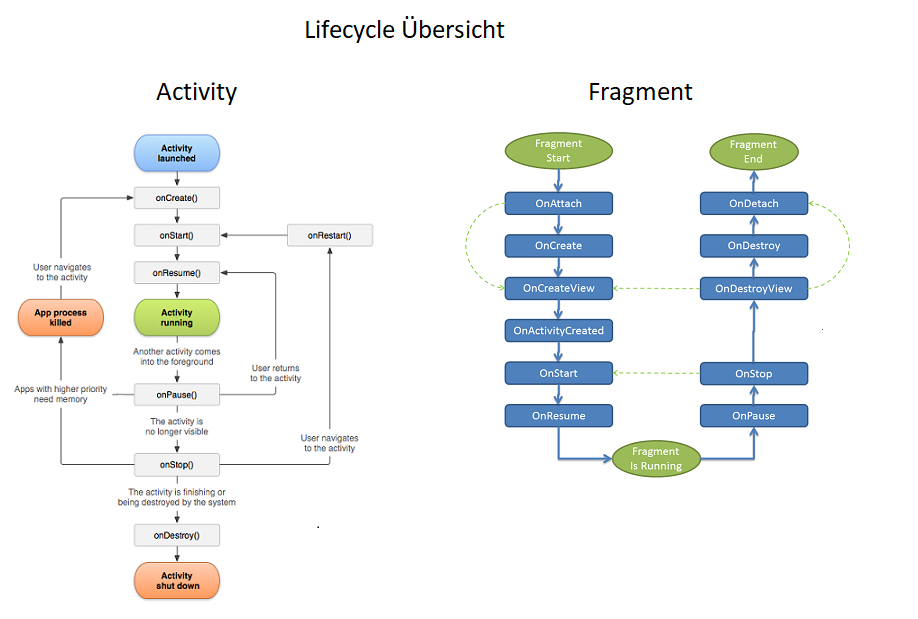
\includegraphics[width=0.8\textwidth]{lifecycleOverview.png}
	\caption[lifecycleOverview]{Prototyp der InVision Vorgabe. Feedback Button f\"ur konkret ausgew\"ahlte Tankstelle}
	\label{fig:lifecycleOverview}
\end{figure}
%https://developer.android.com/reference/android/app/Activity#ActivityLifecycle
%https://docs.microsoft.com/de-de/xamarin/android/platform/fragments/creating-a-fragment

% ----------------------------
\section{H2 Mobility App}
Die App ist f\"ur Besitzer von Wasserstoffautos, also Autos mit einer Brennstoffzelle, gedacht. "Die Brennstoffzelle wird sich durchsetzen"\footnotemark \footnotetext{URL: http://www.spiegel.de/auto/aktuell/wasserstoffauto-die-brennstoffzelle-wird-sich-durchsetzen-a-1235431.html}, ist sich Toyota-Motorenentwickler Gerald Killmann sicher. Daher hat die H2 Mobility Deutschland GmbH \& Co.KG die Firma portrix.net mit der Entwicklung einer App beauftragt die den Nutzern unter anderem das europ\"aische Tankstellennetz anzeigt, die Route zur n\"achstgelegenen Tankstelle anzeigt, eine Feedback f\"ur die Tankstellenbetreiber, Schulungsvideos zum Tankvorgang und viele weitere Funktionen bietet.
Die Entwicklung der App erfolgt nach R\"ucksprache mit dem Vertreter von H2 Mobility und dem f\"ur das Layout verantwortlichen Designer und wird sowohl f\"ur iOS als auch f\"ur Android bei portrix.net programmiert. Features und design-Prototypen werden \"uber das digitale Produkt Design Tool InVision an die Programmierer vermittelt und anschlie\ss{}end umgesetzt. Aufgrund der hohen Komplexit\"at und des Umfangs den die App mittlerweile angenommen hat sich das Erscheinungsbild zwischenzeitlich stark ver\"andert. Das organische anwachsen der Funktionalit\"at ist am Versionskontrollbaum gut zu erkennen, da das Projekt beinahe 20000 commits enth\"alt.

\subsection{Feedback}
\"Uber InVision kam die Vorgabe einen Prototyp zu entwickeln, der es erm\"oglicht einer konkret ausgew\"ahlten Tankstelle per Knopfdruck ein Feedback zu geben.

\begin{figure}[H]
	\centering 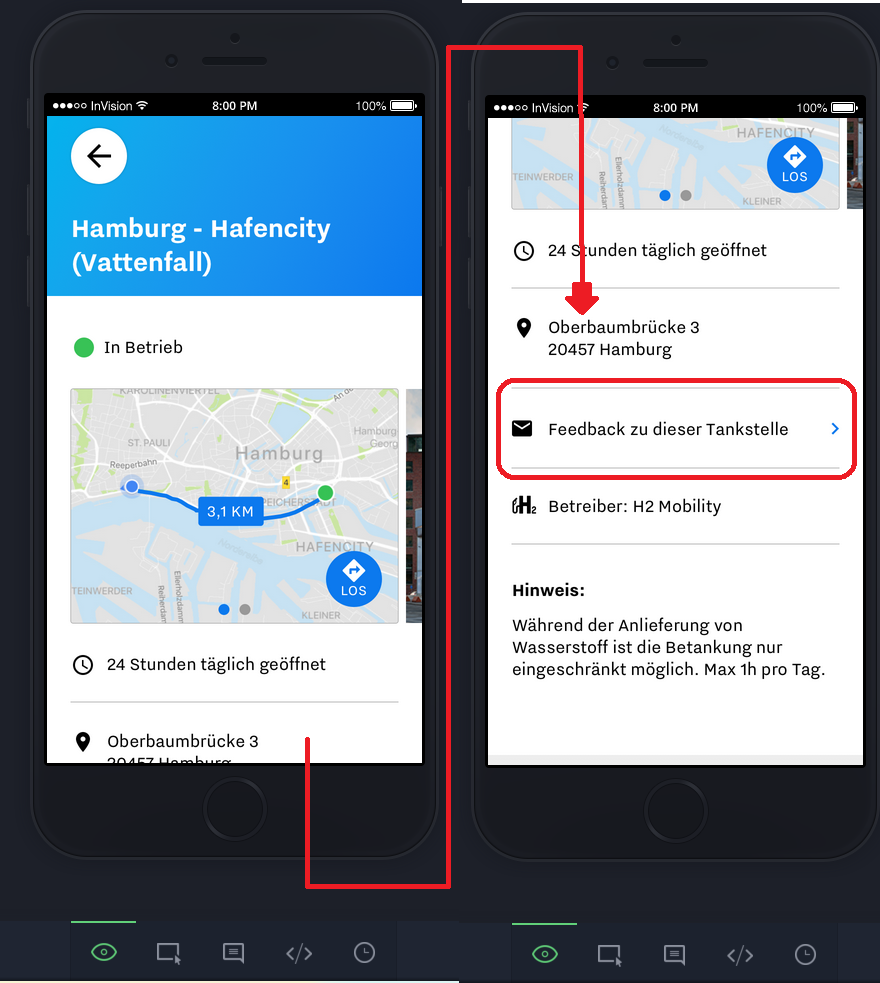
\includegraphics[width=0.8\textwidth]{feedbackPrototyp.png}
	\caption[FeedbackPrototyp]{Prototyp der InVision Vorgabe. Feedback Button f\"ur konkret ausgew\"ahlte Tankstelle}
	\label{fig:FeedbackPrototyp}
\end{figure}
%\footnotetext{URL: https://www.guitarchalk.com/wp-content/uploads/2017/07/electric-guitar-parts.jpg [cited 22 August 2018]}


In der bisherigen Version war es m\"oglich \"uber eine Knopf in der FuelStationsMap.java (MainActivity) das HelpAndFeedback.java (Fragment) aufzurufen und von dort in ein allgemeine Feedback.java (Fragment) zu kommen. Dort l\"asst sich aus einem Spinner, der jede Tankstelle auflistet, eine Tankstelle ausw\"ahlen. Es war also naheliegend den Code zu modifizieren, um aus der FuelStationDetail.java (Activity) direkt in das Feedback.java zu wechseln und die angew\"ahlte Tankstelle direkt im Spinnerfeld anzuzeigen.
Hierzu mussten diverse \"Anderungen vorgenommen werden, da das Feedback.java der darunterliegenden FuelStationsMap.java geh\"ort und in der OnCreate() Methode des Feedback.java eine FuelStationsMap Variable als Context initialisiert wird (\ref{code:onCreate}). Dieser Context gew\"ahrleistet unter anderem das der Spinner im Feedback Fragment mit Tankstellen Daten gef\"ullt werden kann. Der Context macht es allerdings unm\"oglich das Feedback.java von einer weiteren Activity, also der FuelStationDetail.java gestartet wird. Es war daher notwendig die FuelStationDetail.java (Activity) als Fragment nachzubauen. 
Der gew\"unschte workflow wird in Abb.(\ref{fig:inVisionFeedbackPrototyp}) dargestellt.

\begin{figure}[H]
	\centering 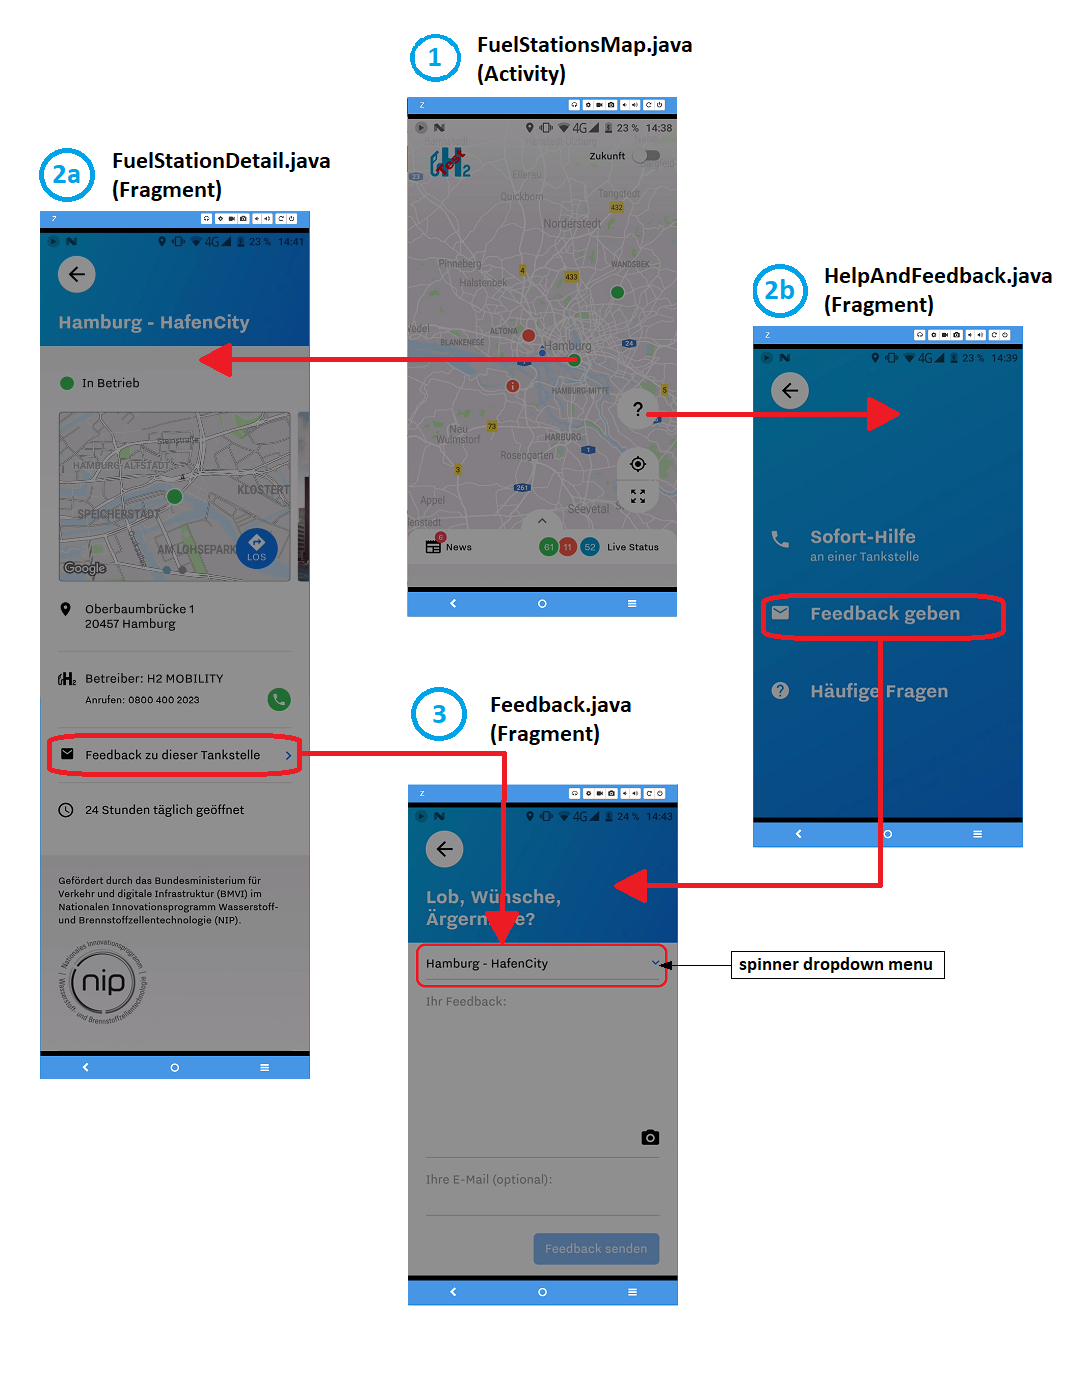
\includegraphics[width=0.8\textwidth]{inVisionFeedbackPrototyp.png}
	\caption[inVisionFeedbackPrototyp]{Workflow der neuen Feedback Funktion}
	\label{fig:inVisionFeedbackPrototyp}
\end{figure}


\fbox{
\lstinputlisting[label={code:onCreate} ,caption={onCreate() Methode der Feedback.java},captionpos=b, language = java,  numbers = left]{program/Feedback.java}
}

Das Layout einer App wird in der zur Activity bzw. Fragment zugeh\"origen .xml Datei definiert. In diesem Fall konnte der meiste Inhalt aus der activity\_fuel\_station\_detail.xml in die neue fragment\_fuel\_station\_detail.xml kopiert und um das gew\"unschte neue Feature erg\"anzt werden (\ref{code:feedbackXml}). 


\fbox{
\lstinputlisting[label={code:feedbackXml} ,caption={Designelement Feedback Button},captionpos=b, language = xml,  numbers = left]{program/fragment_fuel_station_detail.xml}
}

Der Transfer (1 -> 2a) erfolgt durch anklicken eines Tankstellen Markers. Die bisherige Logik rief die FuelStationDetail.java (Activity) auf und musste durch eine Fragment Transaktion ersetzt werden. Zu sehen in Abb.(\ref{code:markerTransaction})
Beim Aufruf von onMarkerClick() wird der angeklickte Marker als Argument �bergeben. Es wird �ber die MapHelper Klasse eine FuelStation Variable station zugewiesen und dessen idx, wenn die station ungleich null ist in ein Bundle gespeichert. Dieses Bundle b wird einem neuen FuelStationDetail Fragment als Argument �bergeben und anschliessend wird mit dem SupportFragmentManager die Fragment Transaktion zum FuelStationDetail mit ausgew�hlter FuelStation.

\fbox{
\lstinputlisting[label={code:markerTransaction} ,caption={Wechsel von FuelStationsMap zu FuelStationDetail},captionpos=b, language = java,  numbers = left]{program/MarkerTransaction.java}
}


Um �ber die Detailansicht der Tankstelle zum gew�nschten Feedback (2a -> 3) zu gelangen muss die ID des FrameLayout lyFeedbackPin deklariert und initialisiert werden und anschlie\ss{}end \"uber einen onClickListener() angeklickt werden. Siehe Abb.(\ref{code:transaction}). Das Prozedere ist dem vorangegangenem \"ahnlich. Der unterschied besteht darin das in der onClick() Methode das Bundle b �ber getArguments() den Marker �bergeben bekommt und an das FeedbackFragment weiterreicht, damit dort das Spinner field menu den Tankstellen namen vorausw�hlen kann. Die eigentliche Transaktion von FuelStationDetail zu Feedback funktioniert nach dem gleichen Muster wie zuvor beschrieben.

\fbox{
\lstinputlisting[label={code:transaction} ,caption={Wechsel von FuelStationDetail zu Feedback},captionpos=bl, language = java,  numbers = left]{program/Transaction.java}
}

%--------------
%design vorgabe von Invision
%direktes Feedback im Fragment
%-----------
\subsection{Opt-Out}
Um das Nutzerverhalten der App zu verbessern werden s\"ammtliche interaktionen des Benutzers mithilfe von Google Analytics registriert. Aufgrund des Europ\"aischen Datenschutzgesetzes muss es dem Benutzer m�glich sein dies zu deaktivieren. Dazu bietet Google Analytics die sogenannte Opt-Out Funktion an. Der "Google Analytics deaktivieren"-Button befindet sich im Impressum (Abb.(\ref{fig:impressum})). Das Impressum ist ein WebView indem die Url des Impressums der H2.Live Webseite aufgerufen und angezeigt wird. Die HTML (\ref{fig:impressum}) enth�lt JavaScript Elemente die in der App ausgelesen und interpretiert werden, wenn der Button gedr�ckt wird.

\begin{figure}[H]
	\centering 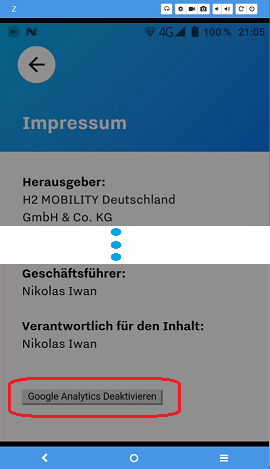
\includegraphics[width=0.4\textwidth]{impressum.png}
	\caption[impressum]{Impressum mit Google Analytics deaktivieren Button}
	\label{fig:impressum}
\end{figure}

\fbox{
\lstinputlisting[label={code:optout} ,caption={Html des Impressums},captionpos=b, language = html,  numbers = left]{program/optout.html}
}

\fbox{
\lstinputlisting[label={code:webview},caption={Interpretation von JavaScript in Android Studio},captionpos=b, language = html,  numbers = left]{program/webview.java}
}


% ----------------------------
\section{LFI App}
super fotografie app
\subsection{Magazin Overview}
neugestaltung der Magazin ansicht
\subsection{Magazin Preview}
Magazin vorschau mit 10 beispielseiten

% ----------------------------
\section{Launcher App}
angesagte Spiegel Tablet
%%---------------------------------------------------------------------------------------------------
% Theory
%---------------------------------------------------------------------------------------------------
\newpage
\chapter{Theory} 
\section{Basics of Electric Guitars}
\subsubsection{Guitar Components}

\begin{figure}[H]
	\centering \includegraphics[width=0.8\textwidth]{banksy.jpg}
	\caption[ElectricGuitar]{Components of an electric guitar\footnotemark}
	\label{fig:ElectricGuitar}
\end{figure}
\footnotetext{URL: https://www.guitarchalk.com/wp-content/uploads/2017/07/electric-guitar-parts.jpg [cited 22 August 2018]}

A regular electric guitar consists of six strings and two or three pickups (\ref{fig:ElectricGuitar}).
Acoustic guitars have a hollow soundboard in which the vibration of the strings resonates. As a consequence, the sound is transmitted to the air. Regular electric guitars have a solid-body and depend on electromagnetic
pickups which are turning mechanical vibrations into an electric signal for further amplification.\\
Before the output signal is provided for the processing by external devices, it can be modified
by the volume and tone controls. The volume controller is a potentiometer that regulates the output voltage.
Tone controls consists of a potentiometer connected in series with a capacitor simply acting as a filter.
%In regard to the main goal of this work, there is no further explanation of the controls necessary.
% Not neary describes cause not part of this thesis


\begin{figure}[H]
	\centering \includegraphics[width=0.5\textwidth]{banksy.jpg}
	\caption[SingleCoil]{Scheme of a single-coil pickup \cite[p 29]{Zollner:2009}}
	\label{fig:SingleCoil}
\end{figure}

For this thesis only passive single coil pickups, as fitted to the majority of electric guitars, are described.
A pickup basically consists of six bar magnets wrapped with a copper-wired coil, see figure (\ref{fig:SingleCoil}).
The magnets produce a stable magnetic field which is disturbed when a string is plucked.
A vibrating string, made of ferromagnetic material, induces an electric Voltage into the coil.\\
According to Faraday's law of induction (see eq. \ref{eq:faraday}) the Voltage $u$ in a wound coil of wire with $n$ turns is proportional to the change of the magnetic flux $\Phi$ over time.


\begin{equation}
u=n \frac{d\Phi}{dt}
\label{eq:faraday}
\end{equation}

\subsubsection{Frequency Range}\label{subsec:FrequencyRange}

The sound from a guitar can be described as a note. Furthermore, every note corresponds to a fundamental frequency.
The fundamental frequencies can be calculated (see eq. \ref{eq:fretFrequencies}).\\
The hearable fundamental frequency $f_{\mathrm{string/fret}}$ depends on the fret played and the frequency $f_{0,\mathrm{string}}$ of the open string that is stroked.
A regular six-string guitar with 24 frets in the standard-tuning (\ref{tab:tableFrequencies}) can generate fundamental frequencies between 82,41\,Hz and 1318,5\,Hz.\\
Besides the fundamental frequencies, an electric guitar produces harmonics at the same time.
Harmonics are integer multiples of the fundamental frequency \cite[p.\,150]{Gorne:2015}. These are overlapped with the fundamental 
frequency in the time domain which leads to the measurable signal form at the output.\\
The total frequency range of an electric guitar is extended by the harmonics up to several kilohertz.
As a limiting factor the total hearable frequency range of a human ear, 16\,Hz to 20\,kHz\,\cite[p.\,28]{Gorne:2015} should be taken into consideration.



\begin{equation}
f_{\mathrm{string/fret}} = f_{0,\mathrm{string}}\cdot \sqrt[12]{2}^{\,\mathrm{fret}}
\label{eq:fretFrequencies}
\end{equation}

\begin{table}[H]
\begin{center}
	\begin{tabular}{|c||c|c|c|c|c|c|}
	\hline 
	\textbf{Open string} & 1(Low) & 2 & 3 & 4 & 5 & 6(High) \\ 
	\hline 
	\textbf{Note} & E & A & D & G & B & E \\ 
	\hline 
	$f_{0,\mathrm{string}}/\mathrm{Hz}$ & 82,41 & 110 & 146,83 & 196,00 & 246,94 & 329,63 \\ 
	\hline 
	\end{tabular} 
\caption[Bla]{Standard tuning of a guitar\footnotemark}
\end{center}
\label{tab:tableFrequencies}
\end{table}
\footnotetext{URL: https://en.wikipedia.org/wiki/Guitar\_tunings [cited 22 August 2018]}




\section{Basics of Audio Engineering}\label{cap:BasicsOfAudio}
\subsubsection{Acoustical Level}

The human ear is not designed for absolute loudness values. The principle of
subjective loudness is based on stimuli-doubling and halving \cite[p.\,3]{Gorne:2015}. Therefore the acoustic
levels are described in logarithmic scale to represent human sensory perception.
It is common to refer to a power of a signal or the intensity of the sound as a "level".
To quantify the sound intensity the most common dimension used is the sound pressure level\,(SPL) $L_{\mathrm{p 0}}$ measured
in decibel.
$L_{\mathrm{p}}$ is defined relative to the smallest sound pressure noticeable of $p_0 = 20 \mu \mathrm{Pa}$ as a reference level (see eq.\,\ref{eq:SPL}).
Table \ref{tab:SPLs} shows a few exemplary sound sources and the resulting SPL at one meter distance.


\begin{equation}
L_{\mathrm{p}} = 20 \mathrm{log} \frac{p}{p_0}\, \mathrm{dB}
\label{eq:SPL}
\end{equation}

\begin{table}[H]
\begin{center}
\begin{tabular}{|c|c||c|c|}
\hline 
\textbf{Sound source} & \textbf{$L_{\mathrm{p}}/\mathrm{dB}$ at 1m} & \textbf{Sound source} & \textbf{$L_{\mathrm{p}}/\mathrm{dB}$ at 1m}  \\ 
\hline 
\hline
Threshold of hearing & 0 & Street traffic & 80 \\ 
\hline 
Quiet rural location at night & 20 & Pneumatic hammer & 100 \\ 
\hline 
Library & 40 & Threshold of pain & 120 \\ 
\hline 
Talking & 60 & Rifle & 140 \\ 
\hline 
\end{tabular} 
\caption[oi]{Example of SPL levels\footnotemark}
\end{center}
\label{tab:SPLs}
\end{table}
\footnotetext{URL: https://www.bsria.co.uk/news/article/acoustic-testing-what-is-actually-measured/ [cited 23 August 2018]}
% calc of Pegel

In audio engineering, the sound levels are defined by electrical levels.
To have a corresponding translation from the acoustic level to the electrical level
volume controls are often designed in a logarithmic scale \cite[p.\,34]{Gorne:2015}.
In addition to that, the electrical levels are labelled with a special index.\\
There are two important voltage levels used as a standard.
The American and Japanese manufactures often use a reference voltage of $u_0$=1\,V measured in
decibel volts (dBV)\,(\ref{eq:dBV}). 
The European standard is defined by a reference voltage of $u_0$=0.775\,V as a holdover from the early telephone standards. It is labelled decibel unloaded (dBu)\,(\ref{eq:dBu}) for a clear separation  from decibel volts.


\begin{equation}
L_{\mathrm{u}} = 20 \mathrm{log} \frac{u}{u_0}\,\mathrm{dBV}
\label{eq:dBV}
\end{equation}

\begin{equation}
L_{\mathrm{u}} = 20 \mathrm{log} \frac{u}{u_0}\,\mathrm{dBu}
\label{eq:dBu}
\end{equation}



\subsubsection{Voltage Bridging}\label{cap:TheoryVoltageBriding}

In audio engineering, the transmission of analog audio signals usually happens by cable.
The audio signals are in the baseband so they are transmitted without modulation.
A transmission from an analog audio signal can be described as the transferring process
from the source device towards the load device.
Impedance matching is a requirement used in the field of radio frequency transmissions to  
avoid reflections in the transmission line. The Goal is to gain maximum power transfer.\\
In audio engineering, the power matching principle is not applied.
For the interconnection of two audio devices, a maximum voltage connection is necessary commonly known
as voltage bridging.\\
The principle can be explained on the basis of a voltage divider (see figure \ref{fig:VoltageMatching}).
For a successful transmission, a much higher load impedance compared to the source impedance is required.
In a worst-case scenario, the input impedance of the load is Z$_2$ $>>$ Z$_1$ which would lead to
no measurable voltage at the load. 
To have an efficient transmission of the signal, the voltage at the load device needs to be maximised.
Most manufacturers adhere to a ratio of Z\,$_{1} \geq$ 5 $\cdot$ Z\,$_{2}$\,\cite[p.\,212]{Gorne:2015}.


\begin{figure}[H]
	\centering 
	\fbox{
	\includegraphics[width=0.75\textwidth]{banksy.jpg}
	}
	\caption[VoltageMatching]{Interconnection of two audio units\,(left) - voltage divider\,(right)\footnotemark}
	\label{fig:VoltageMatching}
\end{figure}
\footnotetext{URL: http://www.sengpielaudio.com/calculator-bridging.htm [cited 23 August 2018]}

\subsubsection{Balanced and Unbalanced transmission}

For the transmission of audio signals, two cable types are commonly used.
Unbalanced cables consist of the centred signal wire and the shield, which is the conductor for the signal return as well.
A shielded cable protects the signal from electromagnetic and radio interference.
This noise rejection is only efficient up to a maximum length of 4,5\,-\,6\,meter, due to the fact that
the wire also acts as an antenna and picks up noise again\footnote{https://ask.audio/articles/music-studio-essentials-understanding-balanced-vs-unbalanced-xlr-cables [cited 25 August 2018]}.
Unbalanced cables are often used to connect an electric guitar or a microphone to an amplifier.
In the domain of consumer audio, they are widely spread.

 
The balanced cable has in contrast to the unbalanced system one additional wire for the signal.
Both wires transmit the same signal with a phase shift of 180 degrees.
In other words, the second wire carries the inverse of the signal.
Along the length of the cable, the two signal wires pick up the same additional noise.
Since the noise parts of the two signals are in phase, both wires can be connected to a differential
amplifier in the receiving device \cite[p.\,490]{Dickreiter:2014}. By calculating the difference of both signals the noise can be eliminated.

Balanced audio systems can carry much longer cable runs compared to an unbalanced cable.
They are used in professional sound systems or in recording studio environment for connections between
amplifiers and mixing consoles.



\subsubsection{Line Level}\label{cap:TheoryLineLevel}

The line standard is distributed in a wide range of applications.
It standardizes the audio transmission in many fields such as
home entertainment, television broadcasting, and professional recording studios.
It describes the nominal level as a ratio for a suitable interconnection between
devices designed for line level.\\
\\
For the consumer audio application (such as CD / DVD Players) the decibel volts (dBV) are used.
The nominal level for consumer audio is specified as -10\,dBV.
In professional audio systems (e.g. mixing tables in television studios) the decibel unloaded (dBu) with
a nominal level of +4\,dBu is standard.

Table \ref{tab:LineLevels} shows the line levels with the corresponding nominal voltages which can be calculated with eq.\,\ref{eq:dBV} and eq.\,\ref{eq:dBu}.

Input and output of the line connections present unequal impedances.
Both designed to ensure a suitable interconnection from a line output to a line input.
The impedance of an input is typically around 10\,k$\Omega$ while the output impedance is usual
around 100\,$\Omega$ to 600\,$\Omega$\footnote{https://en.wikipedia.org/wiki/Line\_level [cited 26 August 2018]}.
Due to the higher input impedance, the signal level is maximised and the current is kept low.

\begin{table}[H]
\begin{center}
\begin{tabular}{|c|c|c|c|c|}
\hline 
\textbf{Application Field} & \textbf{Nominal level} & \textbf{Nominal level, $\mathrm{V}_{\mathrm{RMS}}$}  \\ 
\hline 
\hline 
Consumer audio & -10\,dBV & 0,316 \\ 
\hline 
Professional audio & +4\,dBu & 1,228 \\ 
\hline 
\end{tabular} 
\caption[ui]{Line levels and their approximate nominal voltages}
\end{center}
\label{tab:LineLevels}
\end{table}

\subsubsection{Instrument Level}

Every passive instrument with an output connector for further amplification provides a
different voltage level\,(see table \ref{tab:LineLevels}). Depending on the instrument type, a variety of transducers are used to transform acoustical vibrations an electrical voltage.
This is the reason why there is not one single voltage level valid for all instruments. 

\begin{table}[H]
\begin{center}
\begin{tabular}{|c|c|}
\hline 
\textbf{Type} & \textbf{Output level/ $\mathrm{mV}_{\mathrm{RMS}}$} \\ 
\hline 
\hline
Ribbon microphone & 0,1 \\ 
\hline 
150-Ohm dynamic microphone & 10 \\ 
\hline 
Fender Precision bass pickup & 150 \\ 
\hline 
Humbucker guitar pickup & 200 \\ 
\hline 
Piezo guitar pickup & 0.5 \\ 
\hline 
\end{tabular} 
\caption{Output levels for passive transducers\,\cite{Winer:2012}}
\end{center}
\label{tab:LineLevels}
\end{table}


Though for an electric guitar the range can be limited.
Depending on several parameters like adjustment of the bridge, string cross section and strength of the string-stroke a pickup can produce an output signal between 10\,mV$_{\mathrm{RMS}}$ and 1\,V$_{\mathrm{RMS}}$\footnote{http://www.muzique.com/lab/pick.htm [cited 26 August 2018]}.
The strumming on an open A string of a \textit{Fender Stratocaster} leads to a measured output-voltage about 72\,mV$_{\mathrm{RMS}}$\,(-22\,dBV or -20\,dBu) (see figure \ref{fig:singleCoilVoltage}). Due to the additional harmonics, in this case the oscilloscope calculates the complex waveform as 480,4\,Hz. 
These values can be taken as an assumption for a regular output voltage level of an electric guitar for further calculations.


The output impedance of electric guitars varies caused by the diverse guitar types and tone control settings.
A guitar pickup is a high impedance inductive source commonly in the range of 10\,$\mathrm{k}\Omega$ to 25\,$\mathrm{k}\Omega$\footnote{https://learn.sparkfun.com/tutorials/proto-pedal-assembly-and-theory-guide/theory-of-operations [cited 26 August 2018]}.


\begin{figure}[H]
	\centering \includegraphics[width=0.5\textwidth]{banksy.jpg}
	\caption[singleCoilVoltage]{Single-coil pickup waveform of an open A 110\,Hz (Fender Stratocaster)\,\cite[p.\,27]{Dailey:2014}}
	\label{fig:singleCoilVoltage}
\end{figure}

\subsubsection{Analog Audio Connectors}

For the interconnection of audio devices, several connectors and cables are used.
In the area of analog audio engineering  connectors such as XLR, RCA, and phone connectors (often
called audio jacks) are to be mentioned. With regard to the following chapters, only the pinout of the relevant audio jacks (see figure \ref{fig:Jacks}) is shown in table \ref{tab:pinoutAudioJacks}.


\begin{figure}[H]
	\centering \includegraphics[width=0.25\textwidth]{banksy.jpg}
	\caption[Jacks]{Pinout diagram of a stereo audio jack in TRS standard\footnotemark}
	\label{fig:Jacks}
\end{figure}
\footnotetext{URL: https://robrobinette.com/images/Audio/TRS\_Pinout.jpg [cited 25 August 2018]}

\begin{table}[H]
\begin{center}
\begin{tabular}{|c|c|c|c|}
\hline 
\textbf{ Audio jack} &\textbf{ Pin 1 }& \textbf{Pin 2} & \textbf{ Pin 3} \\ 
\hline 
\hline
6.3\,mm mono & SLEEVE: Ground & TIP: Signal &  - \\ 
\hline 
3.5\,mm stereo & SLEEVE: Ground & TIP: Signal (Left) & RING: Signal (Right) \\ 
\hline 
\end{tabular} 
\caption{Pinout of audio jacks}
\end{center}
\label{tab:pinoutAudioJacks}
\end{table}

\section{Raspberry Pi and Audio-HAT}\label{cap:TheoryPi}

The Raspberry Pi is a single-board computer developed by the Raspberry Pi Foundation.
By March 2017 over 12,5\,million Raspberry Pis were sold, making it one of the best-selling
"general purpose computer" behind Apple Macintosh and Microsoft Windows PCs\footnote{https://www.theverge.com/circuitbreaker/2017/3/17/14962170/raspberry-pi-sales-12-5-million-five-years-beats-commodore-64 [cited 26 August 2018]} .

The first generation "Raspberry Pi 1 Model B" in 2012 came with a processor
speed of 700\,MHz, while the newer processors are running with up to 1,4\,GHz.
For this thesis the widely spread "Raspberry Pi 3 Model B" with a 1,2\,GHz Quad Core Processor is used.
A variety of operating systems like Android Things, Debian or the Debian-based Raspian can be installed 
via the SD-card reader.
Equipped with many onboard interfaces, such as GPIO and display ports, the Pi can be used for a vast number of applications.
\\
A major shortcoming is the analog audio output, which is designed as a 3.5mm audio jack.
It provides a Signal-to-Noise ratio\,(SNR) of 65,5\,dBA\,\cite[pp.\,72-74]{Strom:2015}, which leads to a very weak sound quality.
In addition to that, the Pi is not fitted with an analog audio input.

Therefore Sebastian Albers developed in the context of his bachelor thesis\,\cite{Albers:2017} an Audio-HAT
(Hardware Attached on Top). The HAT extends the Raspberry Pi with professional analog stereo audio in- and output. Also placed on the HAT are the analog-to-digital conversion and the digital-to-analog conversion with a digital word size of 24\,Bit and a maximum sampling frequency of 192\,kHz.The SNR has been improved to 97\,dB\,\cite[p.\,94]{Albers:2017}.
Due to Albers achievements, the Raspberry Pi is therefore capable of digital signal processing.

\begin{figure}[H]
	\centering \includegraphics[width=0.65\textwidth]{banksy.jpg}
	\caption[PiandHAT]{Raspberry Pi Model 3B and Audio-HAT \cite[p.\,65]{Albers:2017}}
	\label{fig:PiandHAT}
\end{figure}



\section{Digital Signal Processing}

For the manipulation or processing of analog signals, the digital signal processing is often used. Due to the greatly reduced prices for microelectronics and mass-production of digital circuits, the 
digital signal processing is widely distributed \cite[p.\,101]{Werner:2010}.\\
Figure \ref{fig:DSPScheme} visualizes the process in the context of digital audio effects\,(DAFX) which are part of this thesis. The analog signal $x(t)$ is a continuous-time signal carrying the information as electric pulses of varying amplitude. For the digital signal representation as a discrete-time signal $x(n)$ of the analog signal, an ADC is needed.
The digitization consists of two steps: sampling and quantization.\\
The DAFX box, representing the digital system, performs a manipulation of the sequence of samples $x(n)$ in this case by halving the values. The processed digital signal $y(n)$ is then passed to the DAC for the reconstruction of the analog signal $y(t)$.

\begin{figure}[H]
	\centering \includegraphics[width=1\textwidth]{banksy.jpg}
	\caption[DSPScheme]{Scheme of digital signal processing \cite[p.\,3]{Zolzer:2002}}
	\label{fig:DSPScheme}
\end{figure}


\subsection{Digital Signals}
\subsubsection{Sampling}
The sampling rate $f_\mathrm{s}$ is the number of samples obtained per second in Hertz.
For the sampling of the analog amplitudes on an equidistant grid along the horizontal time axis, the Nyquist-Shannon sampling theorem (\ref{eq:Nyquist}) must be respected.
It defines that $f_\mathrm{s}$ must be higher than twice the maximum frequency $f_{\mathrm{max}}$ of the analog signal.
If this condition is satisfied, the signal can be reconstructed from its samples.
Not fulfilling the theorem, the sampling could lead to the aliasing effect \cite[p.\,103]{Werner:2010}.

\begin{equation}
f_\mathrm{s} > 2\cdot f_{\mathrm{max}} 
\label{eq:Nyquist}
\end{equation}


\subsubsection{Quantization}

For the amplitudes of the analog signal, discrete values are allocated.
They are represented by numbers $x(n)$ along the vertical axis symbolized by dots\,(see figure \ref{fig:DSPScheme}).
The digital resolution, or the vertical scaling, depends on the defined bit depth.
A higher bit depth leads to a minimized quantization error.
For example, in a 24\,bit representation of sample amplitudes the quantization is in the integer number range between -2$^{24}$ to 2$^{24}$-1.
The maximum digital value is defined as 0 decibels to full scale\,(dbFS). Based on that, the digital amplitude levels can be described in relation to a defined maximum.


\subsubsection{Discrete Fourier transform}

For the conversion of signals from the time-domain to the frequency-domain the 
discrete Fourier function\,(DFT) is used\,(eq. \ref{eq:DFT}). Based on that the calculation of the Fourier
transform of a signal can be done by a computer. The sequence $x(n)$ of $N$ complex numbers is
transformed to the frequency-domain $X(k)$.
In addition to DFT, a more efficient way to perform the transformation is the fast Fourier transform (FFT).
The algorithm is basically just an optimized DFT with a significant reduction of the number of multiplications.
It is a mathematical technique of enormous  technological importance because it allows powerful spectrum analysis on inexpensive microcomputers.\\


\begin{equation}
X(k) =\mathrm{ DFT}[x(n)] = \sum_{n=0}^{N-1} x(n)e^{-j2\pi nk/N}
\label{eq:DFT}
\end{equation}
\begin{center}
$ k=0,1,...,N-1$
\end{center}



\subsection{Digital Systems}

The processing of the digital input signal $x(n)$, provided by the ADC, takes place in the digital system.
An implemented algorithm processes every sample by performing mathematical operations.
The result of the processing is the output signal $y(n)$.


\subsubsection{Impulse Response}

The reaction of a system triggered by a short-time signal is defined as the impulse response\,(see \ref{fig:ImpulseResponse}).
The impulse can be modelled with the Dirac delta function $\delta(n)$ as a test signal.
As a result, the output signal is the impulse response $h(n)$.


\begin{figure}[H]
	\centering \includegraphics[width=1\textwidth]{banksy.jpg}
	\caption[ImpulseResponse]{Impulse response $h(n)$ as a time domain description \cite[p.\,18]{Zolzer:2002}}
	\label{fig:ImpulseResponse}
\end{figure}


\subsubsection{Transfer Function}

In the time-domain, the behaviour of a digital system can be described with the impulse response.
The reaction of the system in the frequency domain can be described as well.
A system can reject, pass and enhance certain frequencies included in the input signal spectrum \cite[p.\,21]{Zolzer:2002}.
The Transfer function (\ref{eq:TransferFu}) describes the frequency domain behaviour.
It results by applying the Z-transform (\ref{eq:ZTrans}) which is mapping the discrete signal into a complex frequency domain representation. At this point, the complex Z plane is not explained in detail because it is not relevant for this thesis.

%\begin{itemize}
%\color{red}
%\item \textbf{\huge Maybe PCM and iS2}
%\end{itemize}

\begin{equation}
X(z) = \sum_{n=-\infty}^{\infty} x(n)\cdot z^{-n}
\label{eq:ZTrans}
\end{equation}

\begin{equation}
H(z) = \sum_{n=-\infty}^{\infty} h(n)\cdot z^{-n}
\label{eq:TransferFu}
\end{equation}

\section{Guitar Effects}

Guitar players often want to highlight their own performance by applying specific sounds.
The manipulation of the guitar sound via tone controls is very limited.
Therefore to enhance the sound, effect units are widely spread.
The units are connected between the guitar output and the input of an amplifier.
Inside the unit the analog or digital signal processing takes place, changing the signal in the time-domain and/or in the frequency domain. A selection of popular guitar effect is depicted in table\,\ref{tab:guitarEffects}. In this section, the delay and distortion are described in more detail.


\begin{table}[H]
\begin{center}
\begin{tabular}{|c|p{10cm}|}
\hline 
\textbf{Effect}  & \textbf{Description} \\ 
\hline 
\hline
Clean &  No effect applied to the signal. Simple pass through \\ 
\hline 
Equalizer & Variation of the total frequency spectrum. Adjusts specific frequency ranges \\ 
\hline
Delay & Time effect. Multiplication of the signal with a changed delayed copy of itself in the time domain.
 Creating an echoing sound \\ 
\hline 
Chorus & Modulation effect. Comparable with the delay but in addition to that the frequency of each tone is modified \\ 
\hline 
Tremolo & Manipulation of the amplitude. Varies volume of the sound very quickly over time\\ 
\hline 
Boost & Increases the output signal of the guitar. Ideally used during solos \\ 
\hline 
Overdrive & Signal amplitude is limited by using soft clipping. Creating a rounded but cropped wave and
a distorted sound \\ 
\hline
Distortion & Signal amplitude is limited by using hard clipping. Leads to a full and saturated sound \\ 
\hline
Fuzz & Signal amplitude is amplified and cut off at the same time. Almost sounds like an overstrained speaker and leads to the most extreme distorted sound\\ 
\hline
\end{tabular} 
\end{center}
\caption{List of popular guitar effects}
\label{tab:guitarEffects}
\end{table}


\subsection{Delay}

In technology, a delay is often associated to be a negative effect in terms of signal transmission or processing. From an artistic point of view, the delay effect can improve the sound experience.
In a comparable way that a sound benefits from a naturally reverberant space, a delay effect unit can create an echoing sound.
A famous example of the usage in popular music is \textit{Pink Floyd - Run like hell} \footnote{D.Gilmour/R.Waters (PinkFloyd) "Run like Hell".\textit{The Wall}. Harvest Records,1980.LP }.
The basic principle of a delay effect unit is shown in figure \ref{fig:DelaySimple}.

The resulting output signal is the addition of the two signal paths: The \textit{Bypass Curcuit} and the \textit{Delay Line}.
Due to the \textit{Bypass Curcuit} the guitar signal is passed forward to the output without any manipulation. Besides that, the \textit{Delay Line} consists of recordings of the input signal and the recordings back from the \textit{Feedback Line}. As a result, the sound is enhanced with a decaying echo.




\begin{figure}[H]
	\centering \includegraphics[width=0.5\textwidth]{banksy.jpg}
	\caption[DelaySimple]{Block diagram of the signal-flow for a typical simple delay-line tied to an electric guitar\,\cite[p.\,124]{Hodgson:2010}}
	\label{fig:DelaySimple}
\end{figure}

\subsection{Distortion}

After the invention of the electric guitar, musicians looked for a way to create a louder and heavier sound. On one hand, they boosted the gain level of the guitar by experimenting with new pickups. On the other hand, they increased the volume inside on an amplifier until the vacuum tubes compressed and distorted the guitar signal. As a result, the distorted sound became one of the most important guitar effects and led to the birth of \textit{Rock and Roll}.
For instance, a typical distortion sound is used in the song \textit{In Bloom} by the band \textit{Nirvana}\footnote{K.Cobain (Nirvana) "In Bloom".\textit{Nevermind}. Geffen Records,1991.LP }.

Any deviation of an output signal from the corresponding input signal is called distortion.
There are two kinds of distortion to be distinguished: Linear and nonlinear (see \ref{fig:nonlinearScheme}).

\begin{figure}[H]
	\centering \includegraphics[width=1\textwidth]{banksy.jpg}
	\caption[nonlinearScheme]{Input and output signals of a linear and nonlinear system \cite[p.\,94]{Zolzer:2002}}
	\label{fig:nonlinearScheme}
\end{figure}


\subsubsection{Linear Distortion}
Linear distortion appears when the processing does not affect the original waveform of the signal but a change in amplitude or phase. A simple example is a volume adjustment with no influence on the tone quality. Also, an equalizer for the amplification and/or attenuation of the frequency range is assigned to the linear systems. In addition to that, they occur by using frequency-dependent amplifiers and capacitive or inductive voltage dividers, which do not produce further harmonics \cite{Sengpiel:2007}.

\subsubsection{Nonlinear Distortion}
A nonlinear system affects an output signal that is strongly shaped. In regard to the distortion effect defined in table \ref{tab:guitarEffects} the method of \textit{hard clipping} is to be mentioned here. Nonlinear distortions are caused by curved characteristic lines of semiconductors and vacuum tubes \cite{Sengpiel:2007}. According to that, these systems create harmonic frequency components that are not part of the input signal.\\

Depending on the symmetry of the components's characteristic lines, different parts of the harmonics are amplified.\\
A symmetrical cubic characteristic line highlights the odd integer multiples of the fundamental frequency $f_1$, thus 3$\cdot f_1$,\,5$\cdot f_1$,\,7$\cdot f_1$ and so on.\\
Unsymmetrical quadratic lines lead to even integer multiples such as 2$\cdot f_1$,\,4$\cdot f_1$,\,6$\cdot f_1$.

\subsubsection{Total Harmonic Distortion}

As an indication for the nonlinearity of a system, the total harmonic distortion\,(THD) is defined.
It specifies the relative amount of harmonics expressed in percentage\,(\ref{eq:THD}) or decibel\,(\ref{eq:THDdb}) and describes the extent of distortion\,\cite{Rohde:2005}.
If the amplitude of the fundamental is $U_1$, and the amplitude of the $n$-th harmonic is $U_i$, then the 
THD for $n$ harmonics can be defined.
A lower THD means a more accurate reproduction of the input signal.\\


\begin{equation}
\mathrm{THD}_{\mathrm{dB}} = 20 \cdot \mathrm{log} \frac{\sqrt{\sum\limits_{i=2}^{n} \cdot {U_i}^2}}{{\sqrt{\sum\limits_{i=1}^{n} \cdot {U_i}^2}}}
\label{eq:THDdb}
\end{equation}

\begin{equation}
\mathrm{THD}_{\%} = 10^{\frac{\mathrm{THD/dB}}{20}} \cdot 100
\label{eq:THD}
\end{equation}

Besides the THD, a much more common method for the evaluation of an audio device performance is the total harmonic distortion plus noise\,(THD+N) measurement. In contrast to the THD, the harmonics are measured - by taking into account the resulting noise (see equation \ref{eq:THDdbplusN}).
As well as the THD measurement the THD+N is expressed as an RMS level.

\begin{equation}
\mathrm{THD}_{\mathrm{dB}} = 20 \cdot \mathrm{log} \frac{\sqrt{\sum\limits_{i=2}^{n} \cdot {U_i}^2 + {U_{noise}}^2}}{{\sqrt{\sum\limits_{i=1}^{n} \cdot {U_i}^2}}}
\label{eq:THDdbplusN}
\end{equation}


					% Kapitel 2: Theory
%%---------------------------------------------------------------------------------------------------
% Analyse
%---------------------------------------------------------------------------------------------------
\newpage
\chapter{Requirements}
% fully working Prototype as standard alone device
% hearable usufull effects, measured !!
% in two sections SW HW

The goal of this thesis is to develop a multi-effects unit for electric guitars.
This device should be able to modify an electric guitar's signal according to the required 
effect. As a deliverable, the result should be hearable and measurable.
Designed as a prototype development this project should also show potential improvements for
further development. 
The requirements are split up into the hardware and software demands.

\section{Hardware}

All components of the unit should be placed in a 19-inch case designed for standardized mounting
in a 19-inch rack.
The unit is supposed to use only one power supply from the 230\,V electricity  grid.
The digital signal processing shall be done by a Raspberry Pi in combination with the Audio-HAT developed by Sebastian Albers \cite{Albers:2017}. 
For the signal in- and output, the device should be equipped with two common standard 6,3\,mm audio jacks on the front panel. That allows an easy interconnection with an electric guitar and a guitar amplifier.
In regard to limit the application range, for this development cycle only input signals from passive six-string electric guitars are to be used. Other instruments like electric basses and keyboards are excluded from testing.
In addition to that, a development of a preamp module is necessary for the adjustment from instrument level to the line level of the Audio-HAT's input. The effect unit itself shall not change the loudness of the signal from input to output.
For the user control, a suitable user interface should be mounted on the front panel.


\section{Software}

To demonstrate the audio signal processing capabilities of the Pi in combination with the Audio-HAT, three exemplary guitar effects should be implemented:
A clean, delay and distortion effect according to the hearable and measurable specifications\,(\ref{tab:guitarEffects}).
To control these effects a menu depending on the signals from the user interface should be implemented.
Required features are:

\begin{center} 
   \begin{varwidth}{4in} 
      \begin{itemize} 
      	 \item Visualize current settings on a display 
         \item Switching to another effect
         \item Change three parameters of the effect
      \end{itemize} 
   \end{varwidth} 
\end{center} 

The unit is not supposed to provide a function to combine the effects with each other.
In order to achieve a good stage performance, the maximum latency of the unit from input to output should not be more than $\Delta$t = 10\,ms.
		% Kapitel 3: Requirements
%%---------------------------------------------------------------------------------------------------
% Design
%---------------------------------------------------------------------------------------------------
\newpage
\chapter{Design}

In this chapter, the design process of the effect unit is described.
Before the single parts of the device are developed, a thorough design phase is reasonable.
The usage of a Raspberry Pi 3 Model B in combination with the Audio-HAT is foreseen (for further explanation see section \ref{cap:TheoryPi}).
In the following sections, the choice of hardware and software in order to fulfil the requirements is explained and reasoned.


% Bild von der ersten Idee
% Placed on Amp usw..
% UML of component functions??

\section{Hardware}

\subsection{Case}
All components of the unit are supposed to be placed in one 19-inch case.
19-inch racks offer the advantage of mounting electronic devices into a standardized frame.
In the field of recording studios or stage engineering, they are commonly used.
Cases are available in different rack units $U$ defining the height.
One $U$ is specified by 1,75inch.
The used 19-inch case has $2U$ to provide enough space for the planned display (see \ref{DesignDisplay}).

% Mounted in Rack 
% 2HE for enough space for display
% Plastic for easy modification
%/ explain this choice


\subsection{Preamp Module} \label{DesignPreamp}

The input- and outputlevel of the Audio-HAT is designed for a reference voltage of 1\,V$_{\mathrm{RMS}}$ = 0\,dBV \cite[p.\,31]{Albers:2017}. As a consequence, the Audio-HAT is developed for the interaction with devices on consumer audio line level\,(see section \ref{cap:BasicsOfAudio}).
Therefore a pre-amplifier\,(preamp) for the amplification from instrument level is reasonable to obtain a higher
digital resolution and less quantization noise at the analog-digital conversion.

In addition to that, a suitable voltage bridging is necessary to gain a maximum voltage level on the HAT input. The existing 10\,k$\Omega$ to 25\,k$\Omega$ output impedance from a regular guitar does not ideally match with the 16,753\,k$\Omega$ \cite[p.\,50]{Albers:2017} input impedance provided by the HAT.


% DAS GEHT !!!!
%\begin{wrapfigure}{r}{0.5\textwidth} 
%  \begin{center}
%    \includegraphics[width=0.35\textwidth]{banksy.jpg}
%  \end{center}
%  \caption{A gull}
%\end{wrapfigure}

The MXR-Micro Amp is a simple but efficient classical effect unit designed as a stompbox\,(figure \ref{fig:MicroAmp}).
It is categorized  as a \textit{Boost} effect, which is a clean volume increaser without any modification of the sound. Taking the advantage of available schematics from the internet\,\cite{ElectroSmash:2017} the Micro Amp is used as a base for the preamp development.

\begin{figure}[H]
	\centering \includegraphics[width=0.35\textwidth]{banksy.jpg}
	\caption[MicroAmp]{MXR Micro-Amp stompbox\footnotemark}
	\label{fig:MicroAmp}
\end{figure} 
\footnotetext{URL: https://www.constantinecruz.com/product/mxr-m133-micro-amp-pedal/ [cited 28 August 2018]}

The Micro Amp is designed in a non-inverting topology originally equipped with the operational amplifier TL061 \cite{Tl061:2015} by Texas Instruments. The main advantage of the TL061 is the very low power consumption, necessary for a battery operating stompbox.
A very low power consumption is not needed, so this part is replaced by the low noise TL071ACP, which is often used for high-fidelity  and audio pre-amplifier applications \cite{Tl071:2017}.\\
Table \ref{tab:OPAmpvergleich} shows a comparison in terms of slew rate $SR$, equivalent input 
noise voltage $V_\mathrm{n}$ and THD to justify this choice.


\begin{table}[H]
\begin{center}
\begin{tabular}{|c|c|c|c|}
\hline 
\textbf{operational amplifier} & \textbf{$SR/ \frac{\mathrm{V}}{\mu \mathrm{s}}$} & $V_\mathrm{n} / \frac{\mathrm{nV}}{\sqrt{\mathrm{Hz}}}$ &\textbf{$\mathrm{THD}_{\%}$} \\ 
\hline 
\hline
TL061 & 3,5 & 42 & no information \\ 
\hline 
TL071ACP & 13 & 18 & 0,003 \\ 
\hline 
\end{tabular}
\caption{Comparsion of TL061 and TL071ACP operational amplifier}
\end{center}
\label{tab:OPAmpvergleich}
\end{table}

Besides the pre-amplification to adjust the guitar signal level for the Audio-HAT, the output signal of the HAT needs to be attenuated. The reduction of the voltage level from consumer audio line level back to instrument level is planned with a simple voltage divider.


% Need to match signals... IN 6.3mm Out 3.5mm
% Albers mentioned Line Level -> better SNR
% Impedance matching
% Same loudness


\subsection{User Interface Module}\label{cap:designUI}

On the front panel of the case, the user interaction takes places. 
The Raspberry provides a 40 pin header for the interaction with external components.
23 of the 40 pins are allocated for the communication with the Audio HAT\,\cite[p.\,99]{Albers:2017}. The remaining 17 pins can be used for the interconnecting with the user interface module via general purpose input/output (GPIO).

\subsubsection{Display} \label{DesignDisplay}

In regard to an easy use, a suitable display is required to visualize the current state of the effect unit.
There is a vast amount of liquid crystal displays\,(LCD) available for the Raspberry Pi such as graphical displays, touch displays or dot-matrix text modules.\\
The main selection criterion is the usability during live stage performances. Touch displays are a bad solution due to "sweaty" hands of a guitarist on stage. Graphical displays, with a resolution of 128x64 pixel or more, are not necessary because there are no complex graphics intend to visualize.
For a simple navigation through the effects a text display is sufficient.
Considering the word lengths to be displayed an appropriate resolution is 2x20 characters.
Due to the difficult light conditions on stage, an LED background light is useful.
\\
\\
For an easy communication with the Raspberry Pi the chosen LCD 202A BL\,\cite{LCD:2016} by Display Visions provides an integrated HD44780 controller. The interaction via GPIO is possible and libraries including pre-developed functions are available on the internet.
The 5\,VDC supply voltage for the display is provided via GPIO.

%\begin{figure}[H]
%	\centering \includegraphics[width=0.35\textwidth]{banksy.jpg}
%	\caption[LCDExample]{LCD 202A BL: LCD-Modul, 2x20 \cite{Missing 40}.}
%	\label{fig:LCDExample}
%\end{figure} 


\subsubsection{Buttons and Switch} 

For the Power ON/OFF control of the effect unit a simple 230\,V rocker switch with an
imprinted I for ON and 0 for OFF is chosen. Besides that, two push buttons are required.
One for the effect selection and the other one for shutting down the Pi.
Both are foreseen to be connected via GPIO with the Pi, so the maximum switching voltage is
in the extra-low voltage range (<120\,VDC). For a convenient usage on stage, the chosen buttons provide
a snap-action mechanism for a tactile and audible feedback provoking a hearable "click".

% Buttons "Snap action" good for user caused by feedback
% switched Voltage / "Gewinde"
% / explain this choice

\subsubsection{Rotary Encoders} 

As required, three parameters of each effect should be adjustable by the user.
The modification of a parameter is simply interpreted as an increment or decrement of a value.
The most user-friendly solutions are potentiometers or rotary encoders.
The use of a potentiometer requires an extensive analog-to-digtal conversion. In addition to that, the
potentiometer has an unavoidable memory effect caused by the turning position of the wiper.
This would lead to implementation issues in terms of default values for the parameters.\\

Hence, KY-040 rotary encoders (see figure \ref{fig:RotaryEncoder}) are used to fulfil the requirements.
Already soldered on a small printed circuit board\,(PCB) and equipped with pull-up resistors, the rotary encoders can be directly connected via GPIO.

\begin{figure}[H]
	\centering \includegraphics[width=0.2\textwidth]{banksy.jpg}
	\caption[RotaryEncoder]{KY-040 rotary encoder module\footnotemark}
	\label{fig:RotaryEncoder}
\end{figure} 
\footnotetext{https://alltopnotch.co.uk/wp-content/uploads/imported/6/Rotary-Encoder-Module-KY-040-Brick-Sensor-Clickable-Switch-Arduino-ARM-PIC-UK-231884393106.JPG [cited 31 August 2018]}

\subsection{Power Supply}

According to the requirements stated before, the unit should be connected with the 230\,V electricity grid.
The unit requires a 230\,V connection equipped with a protection-earth contact, caused by metallic electrically conductive parts\,(e.g. screws) touchable from the outside of the case.
\\
For the design of the power switching supply, the significant criteria are the lower supply voltages needed for the built-in components.
The Raspberry Pi has a micro USB connection for the 5.1\,VDC operating voltage, covering the supply for the user interface via GPIO as well.
The MXR Micro-Amp, on which the preamp module development is based, was originally  designed for a 9-volt battery.
The operational amplifier is running with a bias voltage\,(virtual ground).
According to the specification of the TL071ACP \citep{Tl071:2017} the recommended supply voltage for the total $V_{\mathrm{CC}}$ is between 10\,VDC and 30\,VDC.
Therefore the desired power switching supply requires a minimum output voltage of 10\,VDC.
For the further reduction of the voltage level for the Raspberry Pi, a DC-to-DC converter can be used.
\\
\\
The electric power of the Raspberry Pi is about 5.1\,V\,$\cdot$\,2.5\,A = 12.75\,W \cite{Pi:2005}, the low power consumption of the preamp module can be neglected. Therefore the power switching supply requires a minimum output power about 13\,W.

Table \ref{tab:PowerSupplyChoice} shows the chosen power supplies. The power switching supply MW LRS-35-12 by Mean Well with an output power of 35\,W is generously designed. This is reasonable in regard to possible further extensions such as the integration of a power amplifier. The step-down module LM2596 is designed for the direct connection to the power switching supply output, providing 5\,VDC for the Raspberry Pi.
\\


\begin{table}[H]
\begin{center}
\begin{tabular}{|c|c|c|c|}
\hline 
\textbf{Type}  & \textbf{Input Voltage}  & \textbf{Output Voltage}  & \textbf{Output Current}  \\ 
\hline 
\hline
MW LRS-35-12 & 85 - 264\,VAC   & 12\,VDC &  3\,A \\ 
\hline 
LM2596 & 3 - 35\,VDC & Adjustable 1.5 -35\,VDC &  3\,A \\ 
\hline 
\end{tabular} 
\caption{Specification of used power supplies \cite{MWLRS35:2016}, \cite{DCDC:2017}}
\end{center}
\label{tab:PowerSupplyChoice}
\end{table}

\section{Software}

The Raspberry Pi 3\,B (plus Audio Hat) is the core component of the effect unit, responsible for the control of the main
features such as audio processing and user interaction.
It is an advantage that the interacting components are all available during the development phase.
That allows an efficient hardware-near programming. Therefore it is planned that the whole software implementation is realised directly on the Raspberry Pi with mouse, keyboard and monitor attached to it.\\
Hence, cross-compiling from an external computer is not necessary.

\subsubsection{Operating System}

There are many different OS\,(Operating Systems) available for the Raspberry Pi.
The official distribution \textit{Raspbian OS} is in direct competition to other systems like \textit{Windows 10 IoT Core} or \textit{Ubuntu Mate}.
For the choice of the ideal OS for this thesis, the main focus is on user-friendliness and the availability
of relevant information and tutorials. In addition to that, the OS should provide the fundament for a necessary IDE. The Linux Debian based \textit{Raspbian OS} is the most distributed operating system and supported by the Raspberry Pi foundation. Therefore it is chosen for the software developing process.
% Raspbian is easy

\subsubsection{Programming Language}

As a consequence of the required minimum latency of the audio signal, a fast programming language is reasonable. \textit{C} or \textit{C++} are common solutions in terms of time-critical tasks in close-to-hardware programming. The planned programming language for this project is \textit{C}. The decision is made on the basis of significant advantages like available libraries for the display control and GPIO declaration. Moreover, the Audio-HAT demonstration program by Sebastian Albers \cite{Albers:2017}, which provides a good basis for further implementations, is written in \textit{C}.
% C-Language cau
% - Demo from ALbers avialable in C
% - Minimize Latency
% - Libraries of Components are in C
% - Interrupt commom in Mü controler


\subsubsection{Integrated Development Environment}

As a suitable integrated development environment\,(IDE) the freeware \textit{Geany} is chosen.
Running on Raspbian OS, \textit{Geany} is a simple but efficient program supporting a vast amount of programming languages including C. There are several plugins available, like a useful debugger or a syntax highlighting function. In fact, the program operates with very short load times, ideal for a hardware-near programming during test phases.
% Available for Rasp
% IDE Geany
% Freeware
% proggraimn lang include C
% debugger  ans extensions




					% Kapitel 4: Design
%%---------------------------------------------------------------------------------------------------
% Realisierung
%---------------------------------------------------------------------------------------------------
\newpage
\chapter{Implementation}

In this chapter, the implementation phase is described in detail. After the fundamental design of the effect unit, all components are implemented separately in the first place. The following schematics and layouts are saved additionally on the attached CD\,(see \ref{DVD}).
During the realisation of the components, pre-testing approaches are reasonable to set adjustments for a good system performance.  

\section{Hardware Realisation}

\subsection{Preamp Module}

Figure \ref{fig:Preamp_schematic} shows the implemented circuit of the preamp module.
The following descriptions and calculations are partially adopted from the available Analysis\,\cite{ElectroSmash:2017}.

\begin{figure}[H]
\fbox{
	\centering \includegraphics[width=1\textwidth]{banksy.jpg}
	}
	\caption[Preamp_schematic]{Schematic of preamp module}
	\label{fig:Preamp_schematic}
	
\end{figure}


\subsubsection{Power Supply and Interfaces}

Via a direct connection to the power switching supply output, the operating voltage of 12\,VDC is established. The TL071ACP is supplied by the 12\,VDC, whereas a voltage divider creates the needed 6\,VDC
bias voltage to ensure amplification of negative an positive signal amplitudes.

The preamp provides two 6.3\,mm mono audio jacks for the external interconnection of the effect unit, designed as unbalanced connections. A guitar output is supposed to be connected with the \textit{INSTRUMENT\_IN} - a guitar amplifier via \textit{INSTRUMENT\_OUT}.\\
For the unbalanced connection with the Audio-HAT two 3.5\,mm stereo audio jacks are implemented.
Due to the connection of the TIP-Pin only the left channel is used (mono).
The \textit{LINE\_OUT} is connected with the audio input of the HAT, \textit{LINE\_IN} receives the HAT's 
output signal.\\
\\




\subsubsection{Voltage Gain}
The original Micro-Amp is equipped with a gain regulator for an amplification between 0\,dB and 26,2\,dB. For the preamp module a fixed amplification is used, suitable for different passive guitars.
The goal is to raise the instrument level of the guitar to consumer audio line level.  
By a calculation done on a theoretical basis, the voltage gain can be assessed\,(\ref{eq:TheorectialGain}) assuming the RMS nominal levels\,(see section \ref{cap:TheoryLineLevel}).
\\
As a result of a practical pre-testing phase, the implemented voltage gain is set to 10,92\,dB (\ref{eq:ActualGain}). This avoids hearable clipping caused by unexpected voltage peaks of different types of guitar pickups and/or heavy strumming styles.

\begin{equation}
\mathrm{Gain}_{\mathrm{theoretical}}/\mathrm{dB} = 20 \cdot \mathrm{log} \bigg( \frac{0,316\,\mathrm{V}_{\mathrm{RMS}}}{0,072\,\mathrm{V}_{\mathrm{RMS}}} \bigg) \mathrm{dB}  = 12,85\,\mathrm{dB}
\label{eq:TheorectialGain}
\end{equation}

\begin{equation}
\mathrm{Gain}_{\mathrm{implemented}}/\mathrm{dB} = 20 \cdot \mathrm{log} \Bigg( \bigg( 1+ \frac{R_4}{R_5}\bigg) 
\cdot \bigg( \frac{R_7}{R_6+R_7}\bigg) \Bigg) \mathrm{dB}\ = 10,92\,\mathrm{dB}
\label{eq:ActualGain}
\end{equation}

The processed signal provided by the audio output from the HAT needs to be attenuated by the same factor.
A simple voltage divider formed by \textit{R8} and \textit{R9} is used\,(see \ref{eq:Loss}).
The implemented attenuation differs from an expected loss of -10,92\,dB, due to side effects of the Audio-HAT occurred in a practical test\,(see section \ref{cap:TestDistortion}). 

\begin{equation}
\mathrm{Loss}_/\mathrm{dB} = 20 \cdot \mathrm{log}  \bigg(  \frac{R_9}{R_8 + R_9} \bigg)  \mathrm{dB} = -11.04\,\mathrm{dB}
\label{eq:Loss}
\end{equation}

\subsubsection{Voltage Bridging}

In addition to the signal amplification, the required voltage bridging is guaranteed. For the interconnection with the guitar via \textit{INSTRUMENT\_IN} a suitable high input impedance is achieved
(\ref{eq:ZIn}). Provided by the 10$^{12}\,\Omega$ high JFET Input Stage resistance of the TL071ACP \cite{Tl071:2017}.\\

At the \textit{LINE\_OUT} a lower impedance is implemented to ensure maximum voltage transfer towards the HAT's audio input (\ref{eq:Zout}), based on the TL071ACPs internal output resistance of 192\,$\Omega$ according to the specification.\\ Both adjustments fulfil the required ratio between source and load impedance Z\,$_{\mathrm{load}} \geq$ 5 $\cdot$ Z\,$_{\mathrm{source}}$ (see section \ref{cap:TheoryVoltageBriding}).\\
\\
Guitar amplifiers commonly own a very high input impedance about 1\,M$\Omega$\footnote{URL: https://www.soundonsound.com/sound-advice/q-what-are-correct-input-impedances-guitars-and-mics/ [cited 06 September 2018]}. As a consequence the voltage bridging for the attenuation path between \textit{LINE\_IN} and \textit{INSTRUMENT\_OUT} is not further analysed. 


\begin{equation}
Z_{\mathrm{INSTRUMENT\_IN}} = \big( R_1 || R_2\big) \Big| \Big| \big( R_3 || Z_{\mathrm{ in,TL071ACP}}\big) = 5\,\mathrm{M}\Omega
\label{eq:ZIn}
\end{equation}

\begin{equation}
Z_{\mathrm{LINE\_OUT}} =  R_7 \Big| \Big| \big( R_6 || Z_{\mathrm{out,TL071ACP}}\big) = 657,64\,\Omega
\label{eq:Zout}
\end{equation}

\subsubsection{Frequency Response}

The preamp module is also equipped with four passive filters adopted from the MXR Micro-Amp to preserve its typical transparent and clean sound. These filters are not designed to cut-off relevant bass and treble frequency ranges of the characteristic guitar sound, but to eliminate low-frequency hum and harsh harmonics.
Four RC networks are used, designed as high pass or low pass. The objectives of these filters are not further described in the context of this thesis.

\begin{equation}
f_{\mathrm{cutoff},1} = \frac{1}{2\pi \Big( R_2 || (R_3 + Z_{\mathrm{in,TL071ACP}})\Big)} = 0,159\,\mathrm{Hz}
\label{eq:fc1}
\end{equation}

\begin{equation}
f_{\mathrm{cutoff},2} = \frac{1}{2\pi C_2 R_4} = 60,4\,\mathrm{kHz}
\label{eq:fc2}
\end{equation}

\begin{equation}
f_{\mathrm{cutoff},3} = \frac{1}{2\pi C_3 R_5} = 1,532\,\mathrm{Hz}
\label{eq:fc2}
\end{equation}

\begin{equation}
f_{\mathrm{cutoff},4} = \frac{1}{2\pi C_4 R_7} = 0,159\,\mathrm{Hz}
\label{eq:fc2}
\end{equation}


\subsubsection{PCB Design}

The layout of the preamp module is created with the Freeware version of \textit{EAGLE (Easily Applicable Graphical Layout Editor)} by \textit{Autodesk} \footnote{URL: https://www.autodesk.com/products/eagle/overview [cited 06 September 2018]}.
The resulting printed circuit board\,(PCB) layout is depicted in figure \ref{fig:Preamp_PCB}.
For the mechanical mounting of the preamp module four drill holes with the nominal diameter of 3\,mm are foreseen. In addition to that, the 6.3\,mm Audio jacks protrude over the edge for the direct mechanical coupling with the front panel of the case.\\
The assembled board is shown in figure \ref{fig:Preamp_Photo}.



\begin{figure}[H]
	\centering \includegraphics[width=0.75\textwidth]{banksy.jpg}
	\caption[Preamp_PCB]{PCB layout of preamp module}
	\label{fig:Preamp_PCB}
\end{figure}


\begin{figure}[H]
	\centering \includegraphics[width=0.75\textwidth]{banksy.jpg}
	\caption[Preamp_Photo]{Photo of preamp module}
	\label{fig:Preamp_Photo}
\end{figure}
% Used Eagle / maybe mention used own Parts
% show BRD and PHOTO
\newpage
\subsection{User Interface Module}\label{cap:hardwareUI}

For the connection of the chosen interface components\,(see section \ref{cap:designUI}) the 40 pin-header of the Raspberry Pi is used. As mentioned before 23 of 40 Pins are allocated by the Audio-HAT, thus 17 pins are available.\\
Acting as an intermediate element a module is implemented to unify common voltage potentials and provide enough space for needed additional resistors.
The Pi and the user interface periphery is connected via jumper cables with the module.
Figure \ref{fig:UI_schematic} shows the implemented board with the pin headers \textit{X1} to \textit{X6} for the periphery and \textit{X7} for the direct forwarding towards the Raspberry Pi.

\begin{figure}[H]
\centering 
	\fbox{
	\includegraphics[width=0.7\textwidth]{banksy.jpg}
	}
	\caption[UI_schematic]{Schematic of user interface module}
	\label{fig:UI_schematic}
	
\end{figure}

\subsubsection{Rotary Encoders and Buttons}

The incremental rotary encoders KY-040 are equipped with five contacts. Besides the \textit{+} and \textit{GND} for the voltage supply, the two encoder signals \textit{CLK} and \textit{DT} are used to interpret the rotation direction.
The usage of the \textit{SW} contact, which is delivering a high signal when the encoder is pressed, is left out.\\
\\
For the interconnection of the rotary encoders and the buttons, suitable pull-up and/or pull-down resistors are
necessary. The appropriate debouncing is done on the software side.
The onboard PCB of the rotary encoders already provides two 10\,k$\Omega$ pull-up resistors for the encoder contacts \textit{CLK} and \textit{DT}.
Hence, \textit{X1} to \textit{X3} can be directly connected with the desired GPIO pin of \textit{X7}.
For the buttons on \textit{X4} and \textit{X5} two 10\,k$\Omega$ pull-down resistors are additionally implemented.

\subsubsection{Display}

The LCD 202A-Module is directly connected to the pin header \textit{X6}. The display generally is operating in 4\,bit or 8\,bit mode. In the context of this effect unit, a high update rate for the display is not required, so the benefit of a faster 8\,bit transfer can be neglected.
Therefore, and due to the limited GPIO pins of the Raspberry Pi, the display is connected in 4\,bit mode (see table \ref{tab:DisplayPins}).\\
For the adjustment of the LED backlight brightness, the resistor $R1$ is applied.
As a result of an experimental test with a potentiometer, a value of 470\,$\Omega$ delivers an appropriate brightness. For the LCD contrast adjustment $R2$ = 4,7\,k$\Omega$ turned out to be a suitable choice.


\begin{table}[H]
\begin{center}
\begin{tabular}{|c|c|c|p{6cm}|}
\hline 
\textbf{Pin} & \textbf{Symbol} & \textbf{Level} & \textbf{Description} \\ 
\hline 
\hline
1 & LED- & --- & Back light cathode \\ 
\hline 
2 & LED+ & --- & Back light anode \\ 
\hline 
3 & D7 & H/L & Data bit 7 \\ 
\hline 
4 & D6 & H/L & Data bit 6 \\ 
\hline 
5 & D5 & H/L & Data bit 5 \\ 
\hline 
6 & D4 & H/L & Data bit 4 \\ 
\hline 
7 & E & H/L & Enable signal \\ 
\hline 
8 & RW & H/L & H : Read mode, L : Write mode \\ 
\hline 
9 & RS & H/L & H : Data signal, L : Instruction signal \\ 
\hline 
10 & VEE &  --- & Input Voltage for LCD contrast \\ 
\hline 
11 & VDD & 5\,V & Supply voltage for logic \\ 
\hline 
12 & VSS & 0\,V & Ground \\ 
\hline 
\end{tabular} 
\end{center}
\caption{Interface pin connections of LCD 202A module \cite{LCD:2016}}
\label{tab:DisplayPins}
\end{table}

% Mention that this Module is necessary
% -> show Circuit and calculations (for resitors)
% LCD Resistors by Poti-Trying
\subsubsection{PCB Design}

The development of the PCB for the user interface module is comparable to the
construction of the preamp module.
Four drill holes with the nominal diameter of 3\,mm allow a tight mechanical coupling with the bottom plate of the case. Figure \ref{fig:UI_PCB} shows the PCB layout created with \textit{EAGLE}. The completely equipped board is depicted in Figure \ref{fig:UI_Photo}.
\begin{figure}[H]
	\centering \includegraphics[width=0.8\textwidth]{banksy.jpg}
	\caption[UI_PCB]{PCB layout of user interface module.}
	\label{fig:UI_PCB}
\end{figure}

\begin{figure}[H]
	\centering \includegraphics[width=0.8\textwidth]{banksy.jpg}
	\caption[UI_Photo]{Photo of user interface module}
	\label{fig:UI_Photo}
\end{figure}
% -> show BRD and PHOTO

\subsection{Construction of complete Unit}

All modules and components are placed inside the 19-inch case. The mounting is realised with fitting screws and nuts, except for the 230\,V power switch and the display which are fixed by a \textit{Snap-In} mechanism.\\
A total schematic of the effect unit is placed in the appendix\,(see figure  \ref{fig:UMLoverall}).



\subsubsection{Wiring of Power Supply}

For a secure and reliable electrical wiring of the 230\,V components, only \textit{H07V-K <VDE>} stranded wires with a diameter of 0,75\,mm$^2$ are used. In addition to that, suitable cable lugs and ferrules are applied as a standard in electrical enclosures.
For the power supply wiring of the extra low voltage components, these security regulations are not mandatory.

\subsubsection{Wiring of Signals}

The control signals are realized with the use of jumper cables, ideally for a fast and easy connection.
The resulting cable harness at pin headers $X1$ to $X6$ of the user interface module is bind together by cable ties. For the interconnection of the 40 pin header $X7$ with the Raspberry Pi, a ribbon cable is used as an ideal solution.

For the transmission of the audio signal from the preamp module to the Audio-HAT and back, unbalanced stereo audio cables are used. Suitable with the 3,5\,mm stereo audio jacks of the preamp module and the HAT its a forward-thinking choice for possible future extensions.
Figure \ref{fig:Unit_Inner} shows the total wiring of the effect unit.

\begin{figure}[H]
	\centering \includegraphics[width=0.9\textwidth]{banksy.jpg}
	\caption[Unit_Inner]{Top view of effect unit (without cover)}
	\label{fig:Unit_Inner}
\end{figure}

\subsubsection{Front Panel}
The placement of the components on the front panel is designed to gain maximum usability\,(figure \ref{fig:Unit_Front}).
The guitar signal input and output jacks are isolated on the left side. The display is centred on the front panel with a symmetrical formation of the rotary encoders below. As a consequence, the user is able to identify the corresponding rotary encoder for the variation of a parameter value.
The remaining components for the user controls are placed on the right side.

\begin{figure}[H]
	\centering \includegraphics[width=0.9\textwidth]{banksy.jpg}
	\caption[Unit_Front]{Frontal view of effect unit (without cover)}
	\label{fig:Unit_Front}
\end{figure}





\section{Software Realisation}

In order to create a better overview, the implemented software can be separated into two elements: user interaction and audio signal processing. Both elements in combination are important to reach the goal of a fully working effect unit. The final program \textit{guitarEffects.c}\,(provided on the attached CD\,\ref{DVD}) is called via the \textit{rc.local} file of the Raspberry Pi, allowing the execution of the program while the Pi boots. Thus the effect unit is fully controlled via the user controls placed on the front panel.


\subsection{Audio Signal Processing}

The \textit{i2cDemo.c} program provided by Sebastian Albers\,\cite{Albers:2017} was originally developed for the demonstration of the signal processing capabilities of the HAT. The program forms a good basis for the implementation for the required guitar effects, by initializing ADC and DAC communication and setting up the audio performance parameters.\\
For the audio processing, the sampling rate $f_\mathrm{s}$ is set to 48\,kHz, fulfilling the demand of the Nyquist-Shannon sampling theorem (see equation \ref{eq:Nyquist}).
To ensure a high digital resolution, the bit depth is defined with 24\,bit.\\
The implementation of the guitar effects extends the \textit{i2cDemo.c} program by hearable and measurable sound changes. The manipulation of single samples is realised by taking advantage of the implemented FIFO\,(first in, first out) data buffer.
The communication between the ADC, DAC and the Raspberry Pi is based on the I$^2$S (Inter-IC Sound) serial bus.
For the left and right audio channel, a Pulse-code modulation (PCM) stream is provided.\\

% 48khz 24 bit 
% Explain sourcecode Principles of every Effekt
% (Refer to Theory Block)
% Describe every Parameter / Adjustment by hearing
% Calculation of Samples (24 Bit, LSB usw)
% hints for futre developers
% (Maybe source Code excerpts)
\subsubsection{Clean}
For the clean effect, the samples are not manipulated. The input samples are simply passed forward to the output.  


\subsubsection{Delay}

As depicted before in the block diagram (see \ref{fig:DelaySimple}) the delay a time-effect. An appropriate storage of input samples and the delayed addition with current input samples lead to the resulting output signal. In order to the requirements, a delay effect with three exemplary parameters is implemented.
Figure \ref{fig:ImplementedDelayBlock} shows the signal-flow graph to visualize the algorithm.
\\
\\
The \textit{level} parameter controls the general influence of the delay effect. As a factor placed at the end of the delay line it adjusts the total loudness of the delayed signal part.\\
For the variation of the fall time of the delayed samples, the \textit{decay} parameter is used.
Placed before the storage of input and delayed samples in the \textit{delayBuffer[]}, the \textit{decay} parameter can take the influence of the feedback path into account.
The actual delay time for every sample is controlled by parameter \textit{time}, defining the distance between the input and delayed sample in the time domain.

\begin{figure}[H]
	\centering \includegraphics[width=0.9\textwidth]{banksy.jpg}
	\caption[ImplementedDelayBlock]{Signal-flow graph of implemented delay effect}
	\label{fig:ImplementedDelayBlock}
\end{figure}

Listing 5.1 shows an source code excerpt of the implemented function \textit{i2sDelayEffect()}.
The parameter values are controlled by the variables \textit{globalCounterParameter} set by the rotary encoders.
For a user-friendly control, the adjustable and displayed values are in the range of 1 to 10.
As a consequence, calculations are necessary for a suitable translation.
Parameter \textit{level} and \textit{decay} are implemented as factors, controlling the height of the amplitude in percentage between 0\,\% and 100\,\% (stepsize = 10\,\%).
The \textit{time} parameter is calculated with the sampling rate $f_\mathrm{s}$ and the fixed value 5000\,(see equation \ref{eq:CalcTime}), which leads to a total value range of 0\,ms to 1040\,ms (stepsize = 104\,ms).

\begin{equation}
\Delta t = \frac{\mathrm{globalCounterParameter} \cdot 5000}{f_\mathrm{s}} 
\label{eq:CalcTime}
\end{equation}



\fbox{
\lstinputlisting[caption={Excerpt of delay implementation},captionpos=b, language = c]{program/Delay.c}
}

\subsubsection{Distortion}

There is a wide range of possibilities to achieve a typical distorted guitar sound.
This distortion effect is implemented according to the description in table  \ref{tab:guitarEffects} and uses hard clipping. It is based on the analog method of placing two diodes antiparallel behind an amplifier connected to the ground. The amplitude of the guitar signal gets cut off by the time it reaches the threshold voltage of the diodes. As a consequence, the hard clipping leads to a very aggressive distorted guitar desired from many guitarists.\\
For this thesis, only one adjustable parameter for the threshold value is implemented for demonstration purposes.

The Audio-HAT is configurated with a bit depth of 24\,bit. According to the specification, the ADC \textit{PCM1864} \footnote{http://www.ti.com/lit/ds/symlink/pcm1864.pdf [cited 10 September 2018]} is equipped with a full-Scale input of 2,1\,V$_{\mathrm{RMS}}$.
So for the digital signal processing, the 0\,dBFS level is assigned to a maximum analog level of 2,969\,V$_{\mathrm{Peak}}$.
The DAC \textit{PCM514} provided the same value as a ground centred output. 
Based on that, the $U_{\mathrm{LSB}}$(voltage of the least significant bit) can be defined with equation \ref{eq:Ulsb}.


\begin{equation}
U_{\mathrm{LSB}} = \frac{U_{\mathrm{FS}}}{2^n}  = \frac{2 \cdot 2,969\,V}{2^{24}} = 3,539x10^{-7}\,\mathrm{V}
\label{eq:Ulsb}
\end{equation}

In a pre-testing phase with electric guitars for a suitable clipping-threshold, the hearable result was the most crucial factor. The distortion stages should vary in the range of 0 to 10 (from clean to slightly distorted and up to strongly distorted). A low threshold produces more hearable distortion by becoming a more square-wave-type signal.
Unfortunately, a linear relation between the thresholds led to a more unbalanced subdivision, in terms of subjective perception.\\
\\
Therefore the look-up table $\mathrm{factor\_table[n]}$ according to equation \ref{eq:LUTCalc} is implemented to get thresholds with a non-linear relation. As a result of a multiplication\,(\ref{eq:sampleValue}) of these factors with the fixed number 50000, sample values can be calculated. These values are representing the threshold voltage\,(see eq.\,\ref{eq:UThres}). 
Table \ref{tab:ThresValues} shows the translation of the $\mathrm{globalCounterParameter}$ controlled by the rotary encoder. Figure \ref{fig:ThresholdMATLAB} illustrates the performed hard clipping for every parameter in the time domain.


\begin{equation}
\mathrm{factor\_table[n]} = 30-9.25\sqrt{\mathrm{globalCounterParameter}}
\label{eq:LUTCalc}
\end{equation}

\begin{equation}
\mathrm{sampleValue} = \mathrm{factor\_table[n]} \cdot 50000
\label{eq:sampleValue}
\end{equation}

\begin{equation}
U_{\mathrm{Threshold}} = U_{\mathrm{LSB}}\cdot \mathrm{sampleValue}
\label{eq:UThres}
\end{equation}

\begin{table}[H]
\begin{center}
\begin{tabular}{|c|c|c|c|}
\hline 
 \textbf{globalCounterParameter} & \textbf{factor\_table[n]} & \textbf{sampleValue} & \textbf{$ \pm U_{\mathrm{Threshold}} /\mathrm{mV}$} \\ 
\hline 
\hline
1 & 20,75 & 1037500 & 367 \\ 
\hline 
2 & 16,62 & 846000 & 299 \\ 
\hline 
3 & 13,98 & 699000 & 247 \\ 
\hline 
4 & 11,5 & 575000 & 203 \\ 
\hline 
5 & 9,32 & 466000 & 165 \\ 
\hline 
6 & 7,34 & 367000 & 130 \\ 
\hline 
7 & 5,53 & 276500 & 98 \\ 
\hline 
8 & 3,84 & 192000 & 68 \\ 
\hline 
9 & 2,25 & 112500 & 40 \\ 
\hline 
10 & 0,75 & 37500 & 13 \\ 
\hline 
\end{tabular} 
\end{center}
\caption{Implemented distortion threshold values}
\label{tab:ThresValues}
\end{table}




\begin{figure}[H]
	\centering \includegraphics[width=0.8\textwidth]{banksy.jpg}
	\caption[Threshold]{Implemented hard clipping for globalCounterParameter 1 to 10}
	\label{fig:ThresholdMATLAB}
\end{figure}

After removing all values above the desired threshold, an adjustment is implemented to set the amplitudes to the same voltage level. The implement common level is lower than the original amplitude of the clean signal. This is necessary because the generated harmonics lead to a subjective louder sound.\\
In a pre-testing phase the adjustment-level is set to $\pm$ 160\,mV$_{\mathrm{Peak}}$. As a result, the distortion effect has a similar subjective loudness compared with the other effects. 

\subsection{User Interaction}

As described in \ref{cap:hardwareUI} all user interface components are connected via GPIO with the Raspberry Pi. Instead of an elaborate \textit{Direct Register Access}, the \textit{WiringPI} \footnote{https://github.com/WiringPi [cited 12 September 2018]} GPIO access library is used for an easy way of setting up, reading and writing the pins.\\
Moreover, \textit{WiringPI} includes an LCD library with helpful functions for the display communication. 

The pins allocated to the buttons and rotary encoders are set up as interrupts. Once requested, the audio processing is changed by an user interaction. As a consequence, the display is updated with the current status.\\
\\
In regard to the requirements, a user-friendly menu for the effect navigation is implemented\,(\ref{fig:Menu}).
After the effect unit is turned on with the \textit{Power ON/OFF} switch, the clean effect is executed. For this effect, no parameters are foreseen.
By pressing the \textit{Switch effect} button a new effect is called.
The display is showing the effect name and the three parameter values starting with the default value 5. These values are changeable by turning the corresponding rotary encoder.
For the delay effect the following parameters are assigned\,(from left to right): \textit{level - decay - time}.\\
Only the left parameter of the distortion effect is used for the threshold adjustment. The remaining can be interpreted as dummies. 
By pressing the \textit{Shut down} button at any time, the Pi can start shutting down. After about 5 seconds the voltage of the power switching supply needs to the interrupted manually by pressing the \textit{Power ON/OFF} switch.

\begin{figure}[H]
	\centering \includegraphics[width=1\textwidth]{banksy.jpg}
	\caption[Menu]{Diagram of user menu}
	\label{fig:Menu}
\end{figure}
% -> Activity Diagram of Menu with User Interaction 		%	(looking for solution)
% Explain User selections
% -> Show PHOTO of every Effect incl. Para Name.




	% Kapitel 5: Implementation
%%---------------------------------------------------------------------------------------------------
% Test
%---------------------------------------------------------------------------------------------------
\newpage
\chapter{Test}

After the implementation, the components and the complete unit itself need to be tested. The results are evaluated particularly with regard to the required features.
Table \ref{tab:equipment} shows the laboratory instruments primary used during the testing phase.
Besides a function generator and an audio analyzer as common sources for input signals, the unit is tested with an electric guitar\,(Stratocaster type - single coil pickups with 6 strings). In combination with a guitar amplifier the subjective auditory impression can be evaluated.

\begin{table}[H]
\centering
\begin{tabular}{ll}
	\hline
	\textbf{Instrument} & \textbf{Type}  \\
	\hline
	Peaktech 3500FG & Function Generator  \\
	Tektronik MSO2024 & Oscilloscope  \\
	Rohde \& Schwarz UPV & Audio Analyzer \\
	Harley Benton ST-20 BK & Electric Guitar \\
	Marshall Park G10 & Combo Guitar Amplifier \\
	\hline
\end{tabular}
\caption{Test equipment}
\label{tab:equipment}
\end{table}




\section{Preamp Module Performance}


The preamp module is tested to the two major demands given in the requirements in the first place:
The voltage level adjustment and the voltage bridging. Measured in the time domain with the oscilloscope, the transition of a sine wave is measured. The input signal is provided by the function generator, representing a signal within the voltage- and fundamental frequency-range of an electric guitar. For the inspection of the voltage bridging, the preamp module is tested with and without a connection to the active Audio-HAT (unloaded and loaded).

\subsubsection{Instrument Level to Line Level}

For the amplification path of the preamp module, an input signal with 108\,mV$_{\mathrm{Peak}}$ at 200\,Hz is used.
The measured transition\,(unloaded) from instrument level to line level has a deviation of 3,12\,\% (\ref{tab:Pre-Amplification}), which can be reasoned by production-related deviations of the used parts. For the interconnection with the Audio-HAT, a high voltage transfer is ensured. The signal amplitude is only slightly attenuated by 4,35\,\% as result of suitable voltage bridging(see figure \ref{fig:unloaded} and figure \ref{fig:loaded}).


\begin{table}[H]
\begin{center}
\begin{tabular}{|c|c|c|c|c|}
\hline 
 $U_{\mathrm{INSTRUMENT\_IN}}/\mathrm{mV}$ & $U_{\mathrm{LINE\_OUT}}/\mathrm{mV}$ & $\mathrm{Gain}_{\mathrm{measured}}$ & $\mathrm{Gain}_{\mathrm{implemented}}$ & $\mathrm{deviation}/$\% \\ 
\hline 
108 & 368 & 3,407 & 3,517 & 3,12 \\ 
\hline 
\end{tabular} 
\end{center}
\caption{Measurement of pre-amplification}
\label{tab:Pre-Amplification}
\end{table}

\begin{minipage}[t]{0.5\textwidth}
\includegraphics[width=\textwidth]{Preamp_timedomain/banksy.jpg}
\captionof{figure}{Pre-amplification (unloaded)}
\label{fig:unloaded}
\end{minipage}
\begin{minipage}[t]{0.5\textwidth}
\includegraphics[width=\textwidth]{Preamp_timedomain/banksy.jpg}
\captionof{figure}{Pre-amplification (loaded)}
\label{fig:loaded}
\end{minipage}


\subsubsection{Line Level to Instrument Level}

As an exemplary input signal for the attenuation path 360\,mV$_{\mathrm{Peak}}$ at 200\,Hz is suitable.
For the adjustment of the signal back to instrument level, a minimal deviation of 0.714\,\%\,(\ref{tab:Attenuation}) is achieved.
This is reasonable due to the non-complex used solution as a voltage divider.
An oscilloscope measurement is depicted in figure \ref{fig:Attenuation}.



\begin{table}[H]
\begin{center}
\begin{tabular}{|c|c|c|c|c|}
\hline 
$U_{\mathrm{LINE\_IN}}/\mathrm{mV}$ & $U_{\mathrm{INSTRUMENT\_OUT}}/\mathrm{mV}$ & $\mathrm{Gain}_{\mathrm{measured}}$ & $\mathrm{Gain}_{\mathrm{implemented}}$ & $\mathrm{deviation}/$\%  \\ 
\hline 
360 & 100 & 0,278 & 0,280 & 0,714 \\ 
\hline 
\end{tabular} 
\end{center}
\caption{Measurement of attenuation}
\label{tab:Attenuation}
\end{table}

\begin{figure}[H]
	\centering \includegraphics[width=0.5\textwidth]{Preamp_timedomain/banksy.jpg}
	\caption[Menu]{Attenuation}
	\label{fig:Attenuation}
\end{figure}

\subsubsection{Frequency Response}
% Frequency response and THD
The Audio Analyzer is used for the measurements of the preamp module in the frequency domain. Figure \ref{fig:PreampFreq} shows the frequency response of the amplification path using a sine sweep between 10\,Hz and 20\,kHz. The characteristic flat frequency response of adopted MXR Micro-Amp design is ensured within the range of the fundamental frequencies between 82,41\,Hz and 1318,5\,Hz\,(see section \ref{subsec:FrequencyRange}).
The curve is damped in the range of higher frequencies. The minimal reduction of 4,5\,\% ( $\widehat{=}$ 16\,mV) can be neglected, so the guitar harmonics are appropriately amplified.


\begin{figure}[H]
	\centering \includegraphics[width=0.8\textwidth]{banksy.jpg}
	\caption[Menu]{Preamp frequency response}
	\label{fig:PreampFreq}
\end{figure}

\subsubsection{Total Harmonic Distortion plus Noise}

For the evaluation of the audio performance, the THD+N is measured with the Audio Analyzer.
As a standard for THD+N measurements, a sine-wave signal of 1\,kHz is used. The amplitude is set to 100\,mV$_\mathrm{RMS}$ representing a realistic output of an electric guitar.
The resulting THD+N of -85.003\,dB (0.006\,\%) indicates a very good performance in regard to the desired application field. 

\begin{figure}[H]
	\centering \includegraphics[width=0.5\textwidth]{banksy.jpg}
	\caption[Menu]{Preamp THD+N}
	\label{fig:PreampTHD}
\end{figure}

\subsubsection{Hearable Results}

In a practical test, the isolated preamp module is verified with the usage of the electric guitar signal.
The amplification path is tested in the first place by connecting the \textit{LINE\_OUT} with an AUX(auxiliary) input of HIFI-Amplifier and with the input of a PC-Soundcard. In both cases, the hearable result is a clean undistorted sound from the subjective point of view.
A possible extension for further developments might be a usage of the consumer audio line level outside of the effect unit.\\ 
\\
In a further test, the \textit{LINE\_OUT} is connected directly with \textit{the LINE\_IN} to test the preamp module as a whole.
According to the defined requirements, the total signal processing shall not change the loudness of the guitar signal.
The module is connected via the \textit{INSTRUMENT\_OUT} jack with the Input of the guitar amplifier.
As a hearable result, the guitar-amp gains the same loudness compared to the direct connection of the guitar (at the same amplifier- and guitar settings). 




\section{Measurement of Guitar Effects}

In the following section, the implemented guitar effects are tested.
During the tests, the unit is exclusively controlled by the user interface module.
Due to the combined usage of all in-build components, these tests can be interpreted as a total system validation. The clean effect does not need to be measured in a separate test. The exact clean sound is included in the distortion test by setting the parameter to 0.


\subsection{Delay}

Based on a practical test using a guitar signal, the delay effect is validated.
The effected signal is measured in the time domain for a direct comparison with the original signal. The measurements do not include all possible permutations of the three parameter values from 0 to 10. To visualize and verify the effect, only one parameter is changed while the others are set to 5 as a default value.
Figure \ref{fig:DelayExemp} shows the measurement for one exemplary parameter setting.
The oscilloscope screenshots of the entire measurements are placed in the appendix\,(see \ref{DelayAppendix}).

\begin{figure}[H]
	\centering \includegraphics[width=0.75\textwidth]{banksy.jpg}
	\caption[Menu]{Delay-measurement with \textit{level=5}; \textit{decay=10}; \textit{time=5}}
	\label{fig:DelayExemp}
\end{figure}


\subsubsection{Time Parameter}

Based on equation \ref{eq:CalcTime} using the sampling rate, the \textit{time} parameter is implemented as the repetition time between the original and the delayed sample. Table \ref{tab:time parameter} shows the measured delays. As a result, the exact implemented stepsize of $\Delta$t=104\,ms is verified. 

\begin{table}[H]
\begin{center}
\begin{tabular}{|c|c|c||c|}
\hline 
\textbf{level} & \textbf{decay} & \textbf{time} & $\Delta$t/ms \\ 
\hline 
\hline
5 & 5 & 0 & 0 \\ 
\hline 
5 & 5 & 5 & 520 \\ 
\hline 
5 & 5 & 10 & 1040 \\ 
\hline 
\end{tabular} 
\end{center}
\caption{Measurement of delay effect - \textit{time} parameter}
\label{tab:time parameter}
\end{table}



\subsubsection{Decay Parameter}

Acting as a factor within the \textit{feedback line} (see figure \ref{fig:DelaySimple}) the \textit{decay} parameter has a direct measurable influence at the fall time. The horizontal oscilloscope cursors capture the time span between the original sample and the last recordable delay. The three measured values depicted in Table \ref{tab:decay parameter} are in an expected linear relation.

\begin{table}[H]
\begin{center}
\begin{tabular}{|c|c|c||c|}
\hline 
\textbf{level} & \textbf{decay} & \textbf{time} & $\Delta$t/ms \\ 
\hline 
\hline
5 & 0 & 5 & 0 \\ 
\hline 
5 & 5 & 5 & 1040 \\ 
\hline 
5 & 10 & 5 & 2080 \\ 
\hline 
\end{tabular} 
\end{center}
\caption{Measurement of delay effect - \textit{decay} parameter}
\label{tab:decay parameter}
\end{table}



\subsubsection{Level Parameter}

For the validation of the \textit{level} parameter, the function generator is used for the production of rectangle pulses.
That allows a more efficient detection of the actual peaks contained in the delayed signal.
For a realistic guitar signal, a pulse length of 100\,ms with 0.11\,V$_{\mathrm{Peak}}$ is configurated.
The Task of the \textit{level} parameter is to control the total influence of the delay effect.
The measurement (\ref{tab:level parameter}) shows a direct impact of the parameter on the height of the first delayed peak. It can be observed a reduction of the subsequent delayed by halving the peaks.


\begin{table}[H]
\begin{center}
\begin{tabular}{|c|c|c||c|c|c|c|}
\hline 
\textbf{level} & \textbf{decay} & \textbf{time} & 1stPeak/mV & 2ndPeak/mV & 3rdPeak/mV & 4thPeak/mV\\ 
\hline 
\hline 
0 & 5 & 5 & - & - & - & - \\ 
\hline 
5 & 5 & 5 & 24 & 14 & - & -\\ 
\hline 
10 & 5 & 5 & 48 & 24 & 12 & 6 \\ 
\hline 
\end{tabular} 
\end{center}
\caption{Measurement of delay effect - \textit{level} parameter}
\label{tab:level parameter}
\end{table}

\subsubsection{Hearable Results}

The delay effect tested with the electric guitar in combination with the amplifier leads to the desired echoing sound. The original clean sound gets enhanced by the delayed signal - adjustable by the three rotary encoders after the preferences of the guitarist.
Audio recordings of the delay effect are placed on the attached CD\,(\ref{DVD}) as WAV files.


\subsection{Distortion}\label{cap:TestDistortion}

The following tests contain measurements in the time and frequency-domain to validate the implemented distortion effect. Due to the implementation of only one adjustable parameter, all parameter values from 1 to 10 are tested.
The total set of measurement-screenshots are presented in the appendix (see section \ref{DistortionAppendix}).


\subsubsection{Clipping Thresholds}


According to a useful and playable distortion effect, the signal amplitude at every distortion stage is adjusted to the same level to achieve the same loudness. 
Therefore after the implemented clipping of the signal amplitude takes place, the signal amplitudes are adjusted.
Figure \ref{fig:Thresholds} shows the results of the exemplary measurement for distortion stages 0, 5 and 10 to visualize the clipping and adjustment process.

\begin{figure}[H]

\begin{minipage}[t]{0.5\textwidth}
\includegraphics[width=\textwidth]{banksy.jpg}
\end{minipage}
\begin{minipage}[t]{0.5\textwidth}
\includegraphics[width=\textwidth]{banksy.jpg}
\end{minipage}

\begin{minipage}[t]{0.5\textwidth}
\includegraphics[width=\textwidth]{banksy.jpg}
\end{minipage}
\begin{minipage}[t]{0.5\textwidth}
\includegraphics[width=\textwidth]{banksy.jpg}
\end{minipage}

\begin{minipage}[t]{0.5\textwidth}
\includegraphics[width=\textwidth]{banksy.jpg}
\end{minipage}
\begin{minipage}[t]{0.5\textwidth}
\includegraphics[width=\textwidth]{banksy.jpg}
\label{fig:Threshold}
\end{minipage}

	\caption[Menu]{Measurement of thresholds\,(left) and adjusted levels\,(right) }
	\label{fig:Thresholds}
\end{figure}

%\captionof{figure}{Implemented hard clipping for ParameterValue 0, 5 and 10.}

For the verification of the implemented clipping thresholds, the part that is responsible for the subsequent signal adjustment is commented out. In addition to that, the oscilloscope is directly connected to the \textit{AUDIO\_IN} and \textit{AUDIO\_OUT} of the HAT to gain unchanged values from the ADC and DAC.
Table \ref{tab:ThresMeasurements} depicts the measured clipping threshold in comparison to the implemented values.\\
As a result, an increasing deviation of $\Delta U$ is observed. The most probable cause is the unfavourable choice of a constant scaling of the y-axis during all measurements. In spite of the inaccuracies caused by the incorrect measuring method, the thresholds could be verified. 

\begin{table}[H]
\begin{center}
\begin{tabular}{|c||c|c|c|c|c|c|c|c|c|c|c|}
\hline 
\textbf{ParameterValue} & 0 & 1 & 2 & 3 & 4 & 5 & 6 & 7 & 8 & 9 & 10 \\ 
\hline 
$U_{\mathrm{Thres,implemented}}\,/\,\mathrm{mV}$ & 400 & 367 & 299 & 247 & 203 & 165 & 130 & 98 & 68 & 40 & 13 \\ 
\hline 
$U_{\mathrm{Thres,measured}}\,/\,\mathrm{mV}$ & 400 & 392 & 328 & 272 & 232 & 200 & 160 & 136 & 104 & 80 & 56 \\ 
\hline 
$\Delta U\,/\,\mathrm{mV}$ & 0 & 25 & 29 & 25 & 29 & 35 & 30 & 38 & 36 & 40 & 43 \\ 
\hline 
\end{tabular} 
\end{center}
\caption{Distortion threshold measurements}
\label{tab:ThresMeasurements}
\end{table}



\subsubsection{THD+N}
For a more quantitative valuation of the resulting distorted sound, the signal needs to be examined on resulting harmonics. The chosen input voltage of 100\,mV$_{\mathrm{Peak}}$ is comparable with a guitar output.\\
Figure \ref{fig:THD_0} and \ref{fig:THD_10} show the two extrema of the implemented distortion.
Within the FFT plot, all harmonics are labelled.\\

\begin{minipage}[t]{0.5\textwidth}
\includegraphics[width=\textwidth]{banksy.jpg}
\captionof{figure}{FFT - ParameterValue 0}
\label{fig:THD_0}
\end{minipage}
\begin{minipage}[t]{0.5\textwidth}
\includegraphics[width=\textwidth]{banksy.jpg}
\captionof{figure}{FFT - ParameterValue 10}
\label{fig:THD_10}
\end{minipage}

Since the original waveform of the input signal is changed by hard clipping, the effect performs a non-linear distortion.
The implemented symmetrical clipping affects the positive and negative amplitude equally. 
As a consequence, the cubical parts of the harmonics are heightened. Thus the odd integer multiples of the fundamental frequency.
\\

The measured THD+N values for every distortion stage are shown in table \ref{tab:THDMeasurements}.
For Parameter value 0 a THD+N of -78,38\,dB results. This value was also identified by Sebastian Albers\,\cite[p.\,81]{Albers:2017}. Based on that, the THD+N increases according to the incremental distortion stages.

\begin{table}[H]
\begin{center}


%\begin{tabular}{|c|c|c|c|c|c|c|c|c|c|c|c|}
% \hline 
%\textbf{ParameterValue} & 0 & 1 & 2 & 3 & 4 & 5 & 6 & 7 & 8 & 9 & 10 \\ 
% \hline 
% THD+N\,/\,dB & -78,38 & -18,88 & -15,08 & -12,94 & -11,62 & -10,5 & -9,76 & -9,08 & -8,53 & -7,96 & -7,66 \\ 
% \hline 
% Deviation\,/\,\% & 0,012 & 11,37 & 17,62 & 22,54 & 26,24 & 29,85 & 32,5 & 35,16 & 37,45 & 39,99 & 41,4 \\ 
% \hline 
% \end{tabular}  

\begin{tabular}{|c||c|c|c|c|c|c|}
 \hline 
\textbf{ParameterValue} & 0 & 1 & 2 & 3 & 4 & 5 \\ 
 \hline 
 THD+N\,/\,dB & -78,38 & -18,88 & -15,08 & -12,94 & -11,62 & -10,5  \\ 
 \hline 
 THD+N\,/\,\% & 0,012 & 11,37 & 17,62 & 22,54 & 26,24 & 29,85\\ 
 \hline
 \hline
 \textbf{ParameterValue} & 6 & 7 & 8 & 9 & 10 &  \\ 
 \hline 
 THD+N\,/\,dB  & -9,76 & -9,08 & -8,53 & -7,96 & -7,66 & \\
 \hline 
 THD+N\,/\,\% & 32,5 & 35,16 & 37,45 & 39,99 & 41,4 &\\
 \hline 
  \end{tabular}
 
\end{center}
\caption{THD+N measurements of every distortion stage}
\label{tab:THDMeasurements}
\end{table}

\subsubsection{Hearable Results}

In the practical scenario, all distortion stages are tested. The division of the single stages offers the guitarist a variety of distorted sounds. The slightly distorted sound at parameterValue 1 is suitable for softer song-passages, while the distortion at parameterValue 10 is going a little over the top, from a subjective point of view.
The default value at parameterValue 5 produces a full and saturated sound appropriate for most rock songs.
In addition to that, the adjusted volume level for all distortion stages is similar to the subjective loudness of the other effects.
Audio recordings of the distortion effect are placed on the attached CD\,(\ref{DVD}) as well.

\section{Maximum Latency}
% calculate reqired max distance,,,and sctual
The measurement of the maximum latency includes all relevant hardware components in the total signal chain. Thus, it is the time span measured between \textit{INSTRUMENT\_IN} and  \textit{INSTRUMENT\_OUT}. In the testing phase, all guitar effects lead to the same result. That is reasonable because all implemented effects are forwarding one input sample to the output as a first step. As a result, a total signal latency of $\Delta$t=1.75\,ms is achieved\,(\ref{fig:latency}).\\
That is a very satisfying result, comparable with the physical delay provoked of an amplifier distance of $\Delta$d= 0,6\,m calculated at the assumption of dry air at 20$^{\circ}$\,celsius (see equation \ref{eq:AmpDistance}). 


\begin{figure}[H]
	\centering \includegraphics[width=0.75\textwidth]{banksy.jpg}
	\caption[Menu]{Maximum latency}
	\label{fig:latency}
\end{figure}

\begin{equation}
\Delta d = c \cdot \Delta t = 343 \frac{\mathrm{m}}{\mathrm{s}} \cdot 1,75\,\mathrm{ms} = 0,6\,\mathrm{m}
\label{eq:AmpDistance}
\end{equation}

						% Kapitel 6: Test

%---------------------------------------------------------------------------------------------------
% Der dritte Teil der Arbeit
%---------------------------------------------------------------------------------------------------
	%---------------------------------------------------------------------------------------------------
% Summary
%---------------------------------------------------------------------------------------------------
\newpage
%\part{Schluss}
%\chapter{Schlussteil}
%Ber�hmte letzte Worte...

\chapter{Summary}
% Redo Intruduction
In this thesis, the goal of a fully working multi-effect unit is accomplished.
A Raspberry Pi used in combination with the Audio-HAT performs the task of digital signal processing.\\
Three exemplary guitar effects are implemented:
A clean effect for an unchanged guitar sound, a delay effect with three adjustable parameters for a variety of echoing sounds and a distortion effect based on hard clipping.
All guitar effects are verified on the basis of measurable and hearable results.

Due to the development of a preamp module, the guitar signal is adjusted in an appropriate way.
Hence, the input signal is amplified for an optimal interconnection with the Audio-HAT providing a THD+N of 0.006\,\%.
The other way around the signal is attenuated for further processing by a guitar amplifier.

The user interface allows the guitar player the total system control.
Consisting of a bright LCD-Text display, rotary encoders and buttons the interface is suitable for stage usage.



\subsubsection{Outlook}
% Outlook: Backpanel
%			- Line out  // mention in Test
The concept of the effect unit offers a vast amount of possible extensions.\\
On the hardware side, the unit can be equipped with a power amplifier, due to the generously designed power switching supply. The back panel leaves enough space for speaker connectors. For the interconnection with other
audio devices like HIFI-Amplifiers or PC-Soundcards, a Line-Out via RCA connector sockets is reasonable.
Suitable nominal voltages on consumer audio line level and impedances are available.
Furthermore, the SW contact of the rotary encoders (high signal when the encoder is pressed) could be used for  extensions of the user controls.

The implemented software can be extended by an arbitrary number of guitar effects.
For further developments the source-code is commented at the relevant lines, highlighting good entry points. To provide a greater user-friendliness, it is reasonable to extend the user menu by displayed parameter names.
As a final step, the combination of different effects might be a good idea to achieve an effect chain.



														
%---------------------------------------------------------------------------------------------------	
% Literaturverzeichnis
%---------------------------------------------------------------------------------------------------		
  \bibliographystyle{IEEEtranN}   % was dinat        		    														% Anpassung an deutsche Zitierweise
                                          														% Alphabetische Sortierung, Abk�rzungen
  \bibliography{literatur/literatur}    %KAY: WAR DRINNEN   														% Literaturverzeichnis
%  \nocite{linux}
\nocite{xmlHtml}
\nocite{json}
\nocite{androidUdemy}
\nocite{javaUdemy}
\nocite{gitlab}
\nocite{javaScript}
\nocite{activity}
\nocite{bestPractice}
\nocite{fragment}
\nocite{Nefzger}
\nocite{Schirmbacher}

			 %KAY: WAR DRINNEN   																		% hier k�nnen alle Schriftst�cke aufgef�hrt werden, die nicht zitiert, aber dennoch nennenswert sind!
  

											

%---------------------------------------------------------------------------------------------------	
% Anh�nge
%---------------------------------------------------------------------------------------------------	
	\appendix  							%KAY: WAR DRINNEN   
	  	\input{chapter/Endpart/Appendix.tex}
% \input{anhang/hilfsmittel/hilfsmittel}															% Anhang A: Hilfsmittel zur Erstellung
																																			% 					dieser Arbeit
%	\input{anhang/quellcode/quellcode}																	% Anhang B: Quellcode

%---------------------------------------------------------------------------------------------------	
% Glossar
%---------------------------------------------------------------------------------------------------	
	\printnomenclature

%---------------------------------------------------------------------------------------------------	
% Stichwortverzeichnis
%---------------------------------------------------------------------------------------------------	
	\printindex
	
%---------------------------------------------------------------------------------------------------	
% Erkl�rung �ber Selbstst�ndigkeit
%---------------------------------------------------------------------------------------------------		
	\asurency	

%--------------------------------------------------------------------------------------------------- 
% Ende des Schriftst�cks
%--------------------------------------------------------------------------------------------------- 
\end{document}
